% Options for packages loaded elsewhere
\PassOptionsToPackage{unicode}{hyperref}
\PassOptionsToPackage{hyphens}{url}
%
\documentclass[
  10pt,
]{article}
\usepackage{amsmath,amssymb}
\usepackage{iftex}
\ifPDFTeX
  \usepackage[T1]{fontenc}
  \usepackage[utf8]{inputenc}
  \usepackage{textcomp} % provide euro and other symbols
\else % if luatex or xetex
  \usepackage{unicode-math} % this also loads fontspec
  \defaultfontfeatures{Scale=MatchLowercase}
  \defaultfontfeatures[\rmfamily]{Ligatures=TeX,Scale=1}
\fi
\usepackage{lmodern}
\ifPDFTeX\else
  % xetex/luatex font selection
\fi
% Use upquote if available, for straight quotes in verbatim environments
\IfFileExists{upquote.sty}{\usepackage{upquote}}{}
\IfFileExists{microtype.sty}{% use microtype if available
  \usepackage[]{microtype}
  \UseMicrotypeSet[protrusion]{basicmath} % disable protrusion for tt fonts
}{}
\makeatletter
\@ifundefined{KOMAClassName}{% if non-KOMA class
  \IfFileExists{parskip.sty}{%
    \usepackage{parskip}
  }{% else
    \setlength{\parindent}{0pt}
    \setlength{\parskip}{6pt plus 2pt minus 1pt}}
}{% if KOMA class
  \KOMAoptions{parskip=half}}
\makeatother
\usepackage{xcolor}
\usepackage[margin=1in]{geometry}
\usepackage{graphicx}
\makeatletter
\def\maxwidth{\ifdim\Gin@nat@width>\linewidth\linewidth\else\Gin@nat@width\fi}
\def\maxheight{\ifdim\Gin@nat@height>\textheight\textheight\else\Gin@nat@height\fi}
\makeatother
% Scale images if necessary, so that they will not overflow the page
% margins by default, and it is still possible to overwrite the defaults
% using explicit options in \includegraphics[width, height, ...]{}
\setkeys{Gin}{width=\maxwidth,height=\maxheight,keepaspectratio}
% Set default figure placement to htbp
\makeatletter
\def\fps@figure{htbp}
\makeatother
\setlength{\emergencystretch}{3em} % prevent overfull lines
\providecommand{\tightlist}{%
  \setlength{\itemsep}{0pt}\setlength{\parskip}{0pt}}
\setcounter{secnumdepth}{-\maxdimen} % remove section numbering
\ifLuaTeX
\usepackage[bidi=basic]{babel}
\else
\usepackage[bidi=default]{babel}
\fi
\babelprovide[main,import]{spanish}
% get rid of language-specific shorthands (see #6817):
\let\LanguageShortHands\languageshorthands
\def\languageshorthands#1{}
\usepackage{setspace}
\doublespacing
\usepackage{booktabs}
\usepackage{longtable}
\usepackage{array}
\usepackage{multirow}
\usepackage{wrapfig}
\usepackage{float}
\usepackage{colortbl}
\usepackage{pdflscape}
\usepackage{tabu}
\usepackage{threeparttable}
\usepackage{threeparttablex}
\usepackage[normalem]{ulem}
\usepackage{makecell}
\usepackage{xcolor}
\ifLuaTeX
  \usepackage{selnolig}  % disable illegal ligatures
\fi
\usepackage{bookmark}
\IfFileExists{xurl.sty}{\usepackage{xurl}}{} % add URL line breaks if available
\urlstyle{same}
\hypersetup{
  pdftitle={Trabajo Práctico Final},
  pdfauthor={Econometría},
  pdflang={es-ES},
  hidelinks,
  pdfcreator={LaTeX via pandoc}}

\title{Trabajo Práctico Final}
\author{Econometría}
\date{}

\begin{document}
\maketitle

\renewcommand{\figurename}{Figura}

\begin{center}
    \vspace*{0.5cm}
    \Huge\textbf{Modificaciones para el índice de desarrollo humano}
    
    \vspace{4cm}
    
\includegraphics[width=0.2\textwidth]{logo_fceye.png}
  
    \vspace{0cm}
    \large{Facultad de Ciencias Económicas y Estadística, Universidad Nacional de Rosario}
    
    \vspace{0.5cm}
    \large{Alfonsina Badin, Ailen Salas, Augusto Raynaudo, Camila Matellicani, Julián L'heureux, Sofia Giaquinta}
    
    \vspace{0.5cm}
    \large{Junio 2024}
    
\end{center}

\clearpage

\section{Introducción}\label{introducciuxf3n}

El desarrollo humano es un aspecto súmamente importante para la vida de
las personas y, a nivel país, su nivel es indicador de ciertas
características del territorio, de acciones políticas y las
oportunidades que alcanza. Este se identifica con la idea de ampliar la
riqueza de la vida humana, y no simplemente la riqueza de la economía en
la que viven los seres humanos. Es un enfoque centrado en las personas,
en sus oportunidades y opciones\footnote{Fuente:
  \href{https://hdr.undp.org/about/human-development}{\textcolor{blue}{\underline{Human Development Reports, United Nations Development Programme.}}}.}.

En lugar de dar por sentado que el crecimiento económico conducirá
automáticamente a un mayor bienestar para todas las personas, el
desarrollo humano se enfoca en mejorar sus vidas en un sentido más
amplio, haciendo del crecimiento de los ingresos un medio para el
desarrollo, más que un fin en sí mismo. Bajo esta premisa, se tienen en
cuenta también aspectos que impliquen desarrollar las capacidades de las
personas, brindando la oportunidad y la libertad de utilizarlas, sin
insistir en que las aprovechen.

En 1990 calcula por primera vez el Programa de las Naciones Unidas para
el Desarrollo un indicador del desarrollo humano bajo la definición
mencionada, denominado Índice de Desarrollo Humano (IDH). Este es un
indicador compuesto, extensamente utilizado a nivel internacional, que
relaciona tres dimensiones para dar cuenta del grado de oportunidad
efectiva de expandir las capacidades de las personas: una vida larga y
saludable, el acceso al conocimiento y el tener un nivel estándar de
vida decente. Es una forma de obtener el promedio de los logros de un
área geográfica específica.

Para calcularlo, se toman las variables esperanza de vida, años
esperados de escolaridad, años promedio de escolaridad y producto bruto
nacional (PNB) per cápita de cada país. Se propone cuestionar el uso de
estas variables o si es necesario incluir nuevas en el cálculo, ya que
gracias a la facilidad que Internet ofrece, se podrían tener en cuenta
nuevas medidas de fácil acceso.

El objetivo principal de la presente investigación es proponer una
modificación para el IDH de forma que refleje, en un sentido más
integrado, la naturaleza de cada país en relación al desarrollo humano.
Dada la definición de desarrollo humano antes mencionada, se propone
tener en cuenta para el cálculo del IDH también aspectos sobre la
sociedad, la discriminación, los derechos, la calidad de vida,
desigualdades y las libertades civiles.

\pagebreak

\section{Índice de desarrollo
humano}\label{uxedndice-de-desarrollo-humano}

El IDH se calcula como una media geométrica de índices que representan a
las tres dimensiones estudiadas: una vida larga y saludable, el
conocimiento y un nivel de vida decente.

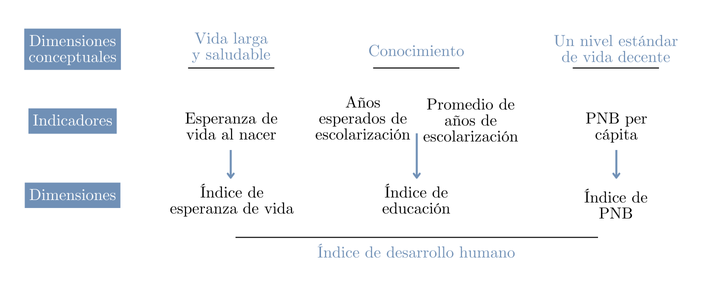
\includegraphics{diagrama1.png}

\[IDH = \Bigl(\text{Índice de esperanza de vida}\times\text{Índice de educación}\times\text{Índice de ingreso}\Bigl)^{1/3}\]

Al considerarse la media geométrica, un mal desempeño en cualquiera de
los componentes se refleja directamente en el valor del índice y no
existe sustitutibilidad perfecta entre ellos. Así, se captura cuán
equilibrado es el desempeño de un país en los tres ámbitos.

Todos estos índices de dimensión se calculan de la siguiente forma:

\[\text{Índice de dimensión}=\frac{\text{valor actual - valor mínimo}}{\text{valor máximo - valor mínimo}}\]

donde los valores mínimo y máximo están definidos para transformar la
variable en un indicador con valores entre 0 y 1 y se llaman ``cero
natural'' y ``objetivo aspiracional'', respectivamente.

\subsubsection{Vida larga y saludable}\label{vida-larga-y-saludable}

La primera dimensión del IDH es vida larga y saludable, que sin dudas
promueve el desarrollo humano y es primordial para mantener un buen
estilo de vida. Actualmente, el indicador que representa este aspecto se
obtiene a partir de la esperanza de vida al nacer: el número medio de
años que un recién nacido podría esperar vivir, si transcurriera su vida
expuesto a las tasas de mortalidad específicas por sexo y edad vigentes
en el momento de su nacimiento, para un año concreto, en un país,
territorio o zona geográfica determinados.

Para el cálculo del IDH se transforma la esperanza de vida al nacer en
un índice calculado con el índice de dimensión mencionado anteriormente,
para esto se definen valores mínimos y máximos de la esperaza de vida.
La elección del cero natural para la esperanza de vida es de 20 años y
está basada en evidencia histórica que muestra que ningún país en el
siglo 20 ha tenido una esperanza de vida menor a los 20 años. El valor
máximo u objetivo aspiracional está definido a los 85 años ya que es un
objetivo realista al que muchos países pueden aspirar, especialmente por
las constantes mejoras en las condiciones de vida y los avances médicos.

De esta forma el índice de esperanza de vida se calcula de la siguiente
forma:

\[\text{Índice de esperanza de vida} = \frac{\text{Esperanza de vida al nacer}-20}{85-20}\]

\subsection{Conocimiento}\label{conocimiento}

En representación de la dimensión del conocimiento, se incluye al
cálculo del IDH el índice de educación. Este se calcula como una media
aritmética entre dos indicadores de dimensión para las variables años
esperados de escolaridad y años promedio de escolaridad.

Los años esperados de escolaridad refieren al número de años de
escolaridad que puede esperar recibir un niño en edad de comenzar la
escuela, si los patrones vigentes de las tasas de matriculación por edad
se mantienen a lo largo de su vida. Y los años medios de escolaridad son
el número promedio de años de educación recibidos por las personas de 25
años o más, calculado a partir de los niveles de logros educativos
utilizando la duración oficial de cada nivel.

Resulta necesario aclarar que para la rama del conocimiento, al tomarse
dos indicadores en vez de uno, primero se calcula el índice de dimensión
de ambos y, a continuación, se obtiene la media aritmética de los dos
índices resultantes.

\[\text{Índice de años esperados} = \frac{\text{Años esperados de escolaridad}-0}{18-0}\]

\[\text{Índice de años medios} = \frac{\text{Años medios de escolaridad}-0}{15-0}\]

Las sociedades pueden subsistir sin educación formal, lo que justifica
la educación mínima de 0 años. El máximo de años esperados de
escolaridad, 18, equivale a la obtención de un máster en la mayoría de
los países. El máximo de años medios de escolaridad, 15, es el máximo
previsto de este indicador para 2025.

El índice de educación queda definido entonces como la media aritmética
de los índices mencionados:

\[\text{Índice de educación} = \frac{\text{Índice años esperados de escolaridad}+\text{Índice años medios de escolaridad}}{2}\]

\subsection{Nivel estándar de vida
decente}\label{nivel-estuxe1ndar-de-vida-decente}

Se considera que un nivel estándar de vida se puede alcanzar cuando la
nación en la que se reside tiene un alto producto bruto interno per
cápita, que refiere al valor monetario de la producción de bienes y
servicios de demanda final de un país o región durante un período
determinado para cada habitante de la población. Es por eso que el PBI
fue la variable considerada en el cálculo del IDH en un principio.

Sin embargo, a partir del año 2010, para medir el nivel de vida, el
producto nacional bruto (PNB) per cápita reemplaza al producto interno
bruto (PBI) per cápita. Esto se debe a que en un mundo globalizado,
suele haber grandes diferencias entre los ingresos de los residentes de
un país y su producto interno. Parte de lo que ganan los habitantes se
envía al extranjero, algunas personas reciben remesas del exterior y
algunos países reciben considerables flujos de ayuda.

Se define al producto nacional bruto (PNB) per cápita como los ingresos
totales de una economía generados por su producción y la propiedad de
los factores de producción, menos los ingresos pagados por el uso de
factores de producción que son propiedad del resto del mundo,
convertidos a dólares internacionales usando las tasas de la PPA, y
divididos por la población a mitad del año.

Para comparar el estándar de vida entre los países, los datos deben
ajustarse por la paridad del poder adquisitivo (PPA) a fin de eliminar
las diferencias en el valor de un dólar entre países. Se entiende por
paridad de poder adquisitivo (PPA) al tipo de cambio que refleja las
diferencias de precios entre países y permite hacer comparaciones
internacionales del producto e ingreso reales. En la tasa de PPA en US\$
(utilizada en este Informe), US\$1 en PPA tiene el mismo poder
adquisitivo en la economía de cualquier país que US\$1 en los Estados
Unidos de América. Para los datos correspondientes al 2019 se utiliza el
PPA en US\$ base de 2011 para ajustar los valores de PNB per cápita.

Para el cálculo de este índice se considera el logaritmo de los valores
ya que el PNB tiene una distribución asimétrica. Además, una vez
alcanzado determinado nivel de vida se necesitan grandes cambios en el
ingreso para mejorarlo aún más, por lo cual se debe atenuar el efecto
del aumento de ingresos en países más desarrollados.

En el \emph{IDH} se calcula el índice de PNB como

\[\text{Índice}_{PNB} = \frac{ln(PNB) - ln(100)}{ln(75.000)-ln(100)}\]

El bajo valor mínimo para el Producto Nacional Bruto per cápita se
considera en los 100 dólares, el uso de este valor se justifica por la
considerable cantidad de producción de subsistencia y producción no
comercial no medida en economías cercanas al mínimo, que no se captura
en los datos oficiales. Por otro lado, el valor máximo se establece en
75.000 dólares per cápita. Kahneman y Deaton (2010) han demostrado que
prácticamente no hay ganancia en desarrollo humano y bienestar con un
ingreso anual per cápita superior a 75,000 dólares. Actualmente solo
cuatro países (Brunei Darussalam, Liechtenstein, Qatar y Singapur)
superan el techo de ingresos per cápita de 75,000 dólares.

\pagebreak

\section[Otras alternativas al cálculo del IDH]{\texorpdfstring{Otras
alternativas al cálculo del
IDH\footnote{Fuente:
  \href{https://www.undp.org/sites/g/files/zskgke326/files/2023-09/notas_tecnicas.pdf}{\textcolor{blue}{\underline{Cálculo de los índices de desarrollo humano, United Nations Development Programme.}}}.}}{Otras alternativas al cálculo del IDH}}\label{otras-alternativas-al-cuxe1lculo-del-idh2}

A través de los años, las Naciones Unidas definieron diversos índices
intentando ampliar la precisión del IDH original, agregando variables y
modificando cálculos a fines de representar mejor el motivo del
análisis. En esta sección se mencionan algunos de ellos:

\begin{itemize}
\item
  \textbf{Índice de Desarrollo Humano ajustado por la Desigualdad
  (IDH-D)}: El IDH-D es una medida que complementa al Índice de
  Desarrollo Humano (IDH) tradicional al incorporar la desigualdad
  existente dentro de un país. Tiene en cuenta las desigualdades
  existentes en las tres dimensiones: salud, educación e ingresos. Para
  ello, hace uso de la familia de mediciones de desigualdad de Atkinson
  (1970) y fija el parámetro de aversión \(\epsilon\) en uno.
\item
  \textbf{Índice de Desarrollo de Género (IDG)}: El IDG refleja las
  desigualdades entre hombres y mujeres realizando el cálculo de las
  tres dimensiones básicas de desarrollo humano por género, y luego
  calcula una razón entre el IDH de las mujeres y el de los hombres.
\item
  \textbf{Índice de Desigualdad de Género (IDG-D)}: El IDG-D refleja la
  desigualdad en tres dimensiones: salud reproductiva, medida por la
  tasa de mortalidad materna y la tasa de natalidad entre las
  adolescentes; empoderamiento, medido por el porcentaje de regidoras y
  regidores, y la población con al menos algún tipo de educación
  secundaria; mercado de trabajo, medido por la tasa de participación en
  la fuerza de trabajo.
\item
  \textbf{Índice de Pobreza Multidimensional (IPM)}: El Índice de
  Pobreza Multidimensional (IPM) identifica múltiples privaciones
  individuales en materia de educación, vivienda y uso de internet,
  salud y protección social. Cada persona de un determinado hogar se
  clasifica como pobre o no, dependiendo de la cantidad de privaciones a
  las que está sometida su familia.
\end{itemize}

Estos son utilizados como punto de partida de nuestra búsqueda y
propuestas para un nuevo IDH ajustado que integre aspectos sobre la
sociedad, sus derechos y libertades, calidad de vida, desigualdades,
etc.

\pagebreak

\section{Cuestionamiento}\label{cuestionamiento}

Durante la investigación se debate cada una de las dimensiones que
componen el IDH con la finalidad de cuestionarlos e intentar una
reformulación que sea más realista para los tiempos que corren.

Si bien se piensa que el calculo del IDH actual logra reflejar muchas
cuestiones vinculadas a lo que hace que un país se pueda considerar con
mayor o menor desarrollo humano, hay otros aspectos de lo que se define
como desarrollo humano que no son tenidos en cuenta.

Poniendo el foco en la dimensión de una vida larga y saludable, se puede
identificar que en un principio el mismo nombre de esta dimensión no
esta completamente explicado por la variable que se utiliza ya que la
esperanza de vida solo indicaría si las personas tienen una vida larga o
corta, pero no se determina qué tan saludable es. Por esta razón, en
esta dimensión se considera importante incorporar otra variable que
pueda tener en cuenta las condiciones en las que se vive, en cuanto a
salud, en los distintos países.

En segundo lugar, se menciona que no se toma por sentado que el
crecimiento económico conduce a un mayor bienestar para todos sino que
los ingresos se consideran un medio para el desarrollo, más que un fin
en sí mismo. Esto indica que si bien una medida como el Producto
Nacional Bruto podría ser un medio para explicar si un país esta más o
menos desarrollado no podría definir esto por completo, ya que el tener
un valor alto de PNB no garantizaría el bienestar de toda la población.
A partir de esta problemática surge la idea de implementar otra variable
de corrección en esta dimensión para así poder tener en cuenta otras
cuestiones del desarrollo humano para el nivel de vida de las personas.

Por otro lado, la definición de desarrollo humano menciona que este
consiste en ofrecer oportunidades a las personas, no de insistir en que
las aprovechen. Es decir, que las personas tengan la libertad de llevar
a cabo la vida que ellos elijan sin imponerles cómo vivirla. Esto no se
tiene en cuenta actualmente en el indice ya que no se calcula una
dimensión de libertad. Se considera que podría ser una propuesta
adecuada incluir una cuarta dimensión al indice de desarrollo humano que
tenga en cuenta cuestiones relacionadas con la libertad y los derechos
de las personas en su día a día.

\section{Propuestas y modificaciones}\label{propuestas-y-modificaciones}

En esta sección se explica cada una de las modificaciones propuestas
para este nuevo índice, acompañado del razonamiento realizado. Además,
se muestran otras posibles propuestas que se podrían llevar a cabo en
investigaciones futuras o descartadas del presente informe por diversas
razones.

\subsection{Vida larga y saludable}\label{vida-larga-y-saludable-1}

\subsubsection{Debate}\label{debate}

Como se mencionó anteriormente, tener una alta esperanza de vida sin
dudas logra una vida larga, pero no necesariamente saludable. Esta
variable no proporciona información sobre la calidad de vida en el
horizonte de años de vida y si este horizonte se desarrolla con buena
salud o, por el contrario, se desarrolla con alguna discapacidad o
dependencia. Es por esto que se propone hacer uso de la Esperanza de
vida saludable al nacer (o Esperanza de vida en buena salud al nacer)
para cuantificar este aspecto según la cantidad de años de calidad y no
sólo en cantidad de años.

Se considera condición de buena salud a la ausencia de limitaciones
funcionales o de discapacidad ya que las enfermedades crónicas, los
problemas mentales y la discapacidad física aumentan su prevalencia con
la edad y reducen la calidad de vida de las personas que sufren estas
condiciones de salud. La esperanza de vida saludable al nacer es una
medida que combina información de mortalidad y de morbilidad y se
calcula en base al método Sullivan.

El método de Sullivan es un método estadístico que combina la
información de las tablas de mortalidad con datos sobre la prevalencia
de morbilidades o limitaciones en la actividad. Ajustando las tablas de
mortalidad con la prevalencia de morbilidad, se calcula la esperanza de
vida saludable, libre de limitaciones, sumando los años de vida
ajustados para obtener una medida integral de salud poblacional. Este
método proporciona una visión clara de los años que se espera que una
persona viva en buena salud, combinando la cantidad y calidad de vida.

En resumen, la organización mundial de la salud define al cálculo de la
esperanza de vida saludable al nacer de la siguiente manera:

\[HALE_x = \Biggl[\sum_{i=x}^w YWD_i\Biggl] \Bigl/ I_x\]

donde:

\begin{itemize}
\item
  \(YWD_x = L_x (1-D_x)\) son los años vividos sin discapacidad entre la
  edad \(x\) y \(x+5\)
\item
  \(I_x\) es el número de sobrevivientes a las edad \(x\)
\item
  \(L_x\) es el total de años vividos entre la edad \(x\) y \(x+5\) de
  la tabla de vida
\item
  \(D_x\) es la proporción de gente con discapacidad entre los años
  \(x\) y \(x+5\)
\end{itemize}

Además, se evaluó la posibilidad de incorporar al cálculo la esperanza
de vida y de vida saludable a los 60 años para considerar el impacto de
la salud en la población mayor en los distintos países. Sin embargo, se
consideró que utilizar únicamente los indicadores al nacer facilita la
interpretación de la dimensión. A su vez, estas medidas otorgan una
visión más amplia de la longevidad y salud de la población a lo largo de
toda su vida.

\subsubsection{Modificación en el cálculo del
IDH}\label{modificaciuxf3n-en-el-cuxe1lculo-del-idh}

La esperanza de vida saludable al nacer se podría considerar una
variable que contiene más información e identifica mejor a la dimensión
``tener una vida larga y saludable''. Ahora bien, ¿cómo incluirla al
cálculo del IDH? Se han barajado algunas opciones:

\begin{enumerate}
\def\labelenumi{\arabic{enumi}.}
\tightlist
\item
  Reemplazar la esperanza de vida al nacer por la esperanza de vida
  saludable al nacer directamente en el cálculo del índice de salud.
  Para la transformación de dicha métrica en índice se calculó el mínimo
  y máximo de esta variable buscando que sea proporcional con el mínimo
  y máximo de la esperanza de vida al nacer.
\end{enumerate}

\[\min(\text{esp. salud}) = \min(\text{esp. vida})*\frac{\min(\text{esp. salud})}{\min(\text{esp. vida})}\]

Siendo:

\begin{itemize}
\item
  \(\min(\text{esp. salud})\): valor fijado para el cero natural de la
  esperanza de vida saludable al nacer.
\item
  \(\min(\text{esp. vida})\): valor fijado para el cero natural de la
  esperanza de vida al nacer (20 años).
\item
  \(\min(\text{esp. salud})\): valor mínimo observado de la esperanza de
  vida saludable al nacer entre los países evaluados.
\item
  \(\min(\text{esp vida})\): valor mínimo observado de la esperanza de
  vida al nacer entre los países evaluados.
\end{itemize}

De igual manera, se calcula el objetivo aspiracional para la esperanza
de vida saludable al nacer. Y, una vez obtenidos ambos valores, se logra
calcular el índice de la dimensión salud.

\[\text{Índice de dimensión}_{\text{salud}} = \frac{\text{esp. salud}-\min(\text{esp. salud})}{\max(\text{esp. salud})-\min(\text{esp. salud})}\]
En la Figura 1 se puede identificar que los resultados del índice de
salud para los países en estudio con ambas metodologías no presentan
grandes cambios. Se observa que el mínimo del Índice de salud disminuye
con el cálculo propuesto, sin embargo, los datos centrales se posicionan
en el mismo rango y el máximo valor parecería mantenerse.

\begin{figure}
\centering
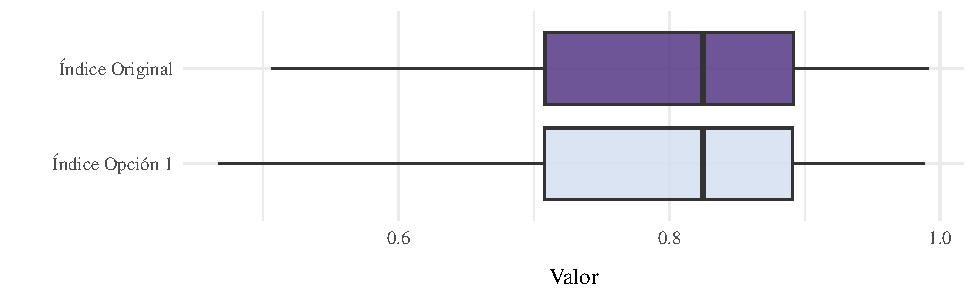
\includegraphics{Informe_files/figure-latex/Figura1-1.pdf}
\caption{Índice de salud obtenido con la metodología original y la
opción 1}
\end{figure}

En la figura \ref{fig:Figura1} se puede identificar que los resultados
del índice de salud para los países en estudio con ambas metodologías no
presentan grandes cambios. Se observa que el mínimo del Índice de salud
disminuye con el cálculo propuesto. Sin embargo, los datos centrales se
posicionan en el mismo rango y el máximo valor parecería mantenerse.

\begin{enumerate}
\def\labelenumi{\arabic{enumi}.}
\setcounter{enumi}{1}
\tightlist
\item
  Tomar ambas variables y promediarlas. Una vez obtenido el promedio se
  calcula el índice de este eligiendo el cero natural y el objetivo
  aspiracional con el criterio utilizado anteriormente.
\end{enumerate}

\[\text{Promedio}=\frac{\text{esp. vida}+\text{esp salud}}{2} \quad \text{Índice de dimensión}_\text{salud} = \frac{\text{Promedio}-\min}{\max-\min}\]

En la Figura 2 se puede identificar que, nuevamente, el cálculo no
parece cambiar notablemente los resultados, disminuyendo el mínimo del
índice de salud respecto al original y manteniendo datos centrales y el
máximo.

\begin{figure}
\centering
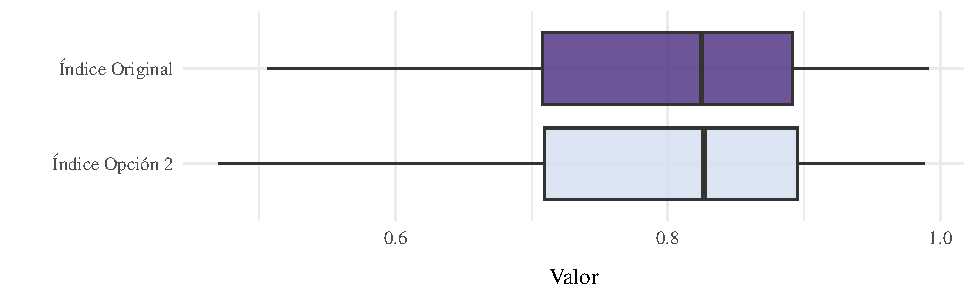
\includegraphics{Informe_files/figure-latex/Figura2-1.pdf}
\caption{Índice de salud obtenido con la metodología original y la
opción 2}
\end{figure}

\begin{enumerate}
\def\labelenumi{\arabic{enumi}.}
\setcounter{enumi}{2}
\tightlist
\item
  Penalizar la esperanza de vida al nacer. Esta opción se lleva a cabo
  transformando la esperanza de vida al nacer y la esperanza de vida
  saludable al nacer en índices y después multiplicándolos. Como era de
  esperarse, esto causa que se penalice mucho el valor de la dimensión
  salud, tal como puede observarse en la Figura 3. Podría pensarse
  distintas ponderaciones para aminorar el peso de la esperanza de vida
  saludable en el cálculo de la dimensión. Sin embargo, para llevarlo a
  cabo se debería contar con un mayor conocimiento sobre la construcción
  de índices y el área de salud, por lo cual se decide no utilizar esta
  opción en el presente informe.
\end{enumerate}

\[\text{Índice de dimensión}_\text{salud}=\text{Índice de esp. vida}\times\text{Índice de esp. salud}\]

\begin{figure}
\centering
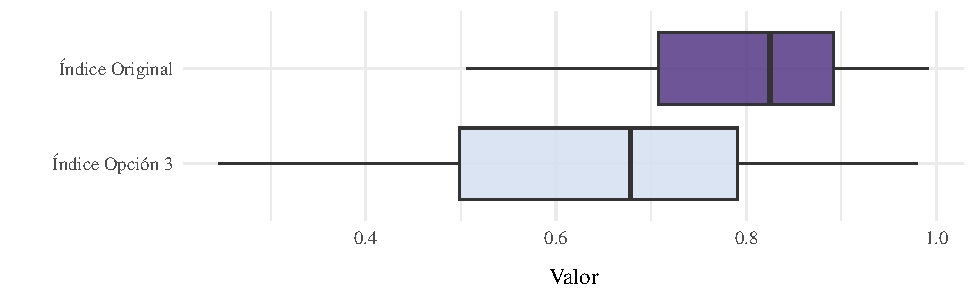
\includegraphics{Informe_files/figure-latex/Figura3-1.pdf}
\caption{Índice de salud obtenido con la metodología original y la
opción 3}
\end{figure}

\begin{enumerate}
\def\labelenumi{\arabic{enumi}.}
\setcounter{enumi}{3}
\tightlist
\item
  Otra alternativa resulta al tomar los índices de esperanza de vida al
  nacer y esperanza de vida saludable al nacer, ya calculados con sus
  respectivos mínimos y máximos, y promediarlos.
\end{enumerate}

\[\text{Índice de dimensión}_\text{salud}=\frac{\text{Índice de esp. vida}+\text{Índice de esp. salud}}{2}\]

En la Figura 4 es evidente que la distribución casi no presenta cambios.
Estos son aún más pequeños que en los casos anteriores dado que se está
utilizando un promedio de los índices lo cuál aminora el efecto de la
nueva variable.

\begin{figure}
\centering
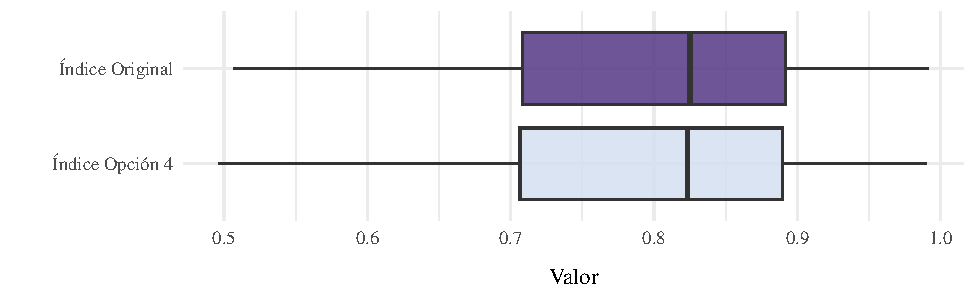
\includegraphics{Informe_files/figure-latex/Figura4-1.pdf}
\caption{Índice de salud obtenido con la metodología original y la
opción 4}
\end{figure}

\begin{enumerate}
\def\labelenumi{\arabic{enumi}.}
\setcounter{enumi}{4}
\tightlist
\item
  Se podría pensar incoporar también la diferencia entre esperanza de
  vida al nacer y la esperanza de vida saludable al nacer de alguna
  manera. Sin embargo, esta idea es más subjetiva ya que valores grandes
  de esta diferencia se pueden considerar como positivos o negativos
  dependiendo de que lado se lo vea. Si bien primeramente se pensó que
  una gran diferencia significaba un país con menor desarrollo ya que
  simbolizaba que muchos de los años vividos eran en mala salud, luego
  se pensó que también esta gran diferencia podía simbolizar que el país
  en cuestión contaba con una gran tecnología y una avanzada medicina
  que hacía que los pacientes vivan más años a pesar de sus condiciones
  de salud. Si el desarrollo se plantea por el lado de avances en la
  humanidad entonces si la diferencia es grande se podría considerar
  como un mayor índice de desarrollo, por lo dicho anteriormente. Dada
  la complejidad y subjetividad del idea propuesta se decidió no
  incorporarla pero se deja plasmada la misma para profundizar este
  análisis en futuras investigaciones.
\end{enumerate}

En base al recorrido realizado, se selecciona a la Opción 1 como la
modificación del cálculo del Índice de Salud. Se consideró que esta
alternativa además de reflejar el cambio que se estaba buscando expresar
en esta componente (priorizar no solo la cantidad si no la calidad),
resulta la de mayor simplicidad a la hora de interpretar la dimensión.

Si bien la distribución de este índice no parece variar demasiado de la
original, hay una variación en el puesto de los países según la
dimensión salud. Esto se evidencia en el Cuadro 1, donde se pueden
visualizar los países con menor esperanza de vida saludable junto al
cálculo del Índice Original y el Índice Modificado. La diferencia entre
las variables Esperanza de vida y Esperanza de vida saludable ocasionan
diferencias en los Índices calculados, que a fin de cuentas generarán el
cambio en el cálculo final del IDH para cada país.

\begin{table}[H]

\caption{\label{tab:unnamed-chunk-1}Resultados del Índice modificado}
\centering
\begin{tabular}[t]{c|c|c|c|c}
\hline
País & Esp. vida & Esp. vida saludable & Índice Original & Índice Modificado\\
\hline
Lesotho & 50.75 & 44.2 & 0.5257385 & 0.4671258\\
\hline
Eswatini & 57.73 & 50.1 & 0.6238308 & 0.5700351\\
\hline
Mozambique & 58.14 & 50.4 & 0.6333231 & 0.5752678\\
\hline
Chad & 59.63 & 52.0 & 0.5116769 & 0.6031754\\
\hline
Guinea-Bissau & 60.22 & 52.6 & 0.6289538 & 0.6136407\\
\hline
\end{tabular}
\end{table}

\subsection{Conocimiento}\label{conocimiento-1}

Antes del año 2010, en el cálculo del IDH se tenían en cuenta las
variables alfabetización y matriculación bruta en la dimensión de
conocimiento. A partir de la publicación del Informe de Desarrollo
Humano en el año 2010, los años promedio de escolaridad sustituyeron a
la alfabetización y la matriculación bruta se replanteó como los años
esperados de escolaridad.

En el 2010, se vio que desde el primer Informe sobre Desarrollo Humano
publicado en 1990, los años promedio de escolaridad habían aumentado en
dos años y la proporción bruta de matriculación, en 12 puntos
porcentuales. Las tasas de alfabetismo, por su parte, habían crecido de
73\% a 84\%. Esto significaba que muchos países habían tenido éxito en
el campo de la enseñanza, al menos según en las mediciones del IDH
convencional. Esto explica una de las principales motivaciones para
realizar los ajustes en el campo de conocimiento.

El alfabetismo y los años de instrucción reflejaban el acceso (o la
falta de acceso) a la educación por parte del segmento de la población
que en su momento habían llegado a la adultez. Por consiguiente, el
progreso registrado quizás no refleje los adelantos recientes en
escolaridad de los jóvenes. Dadas las mejoras mencionadas en educación,
parecía que la falta de habilidades básicas de redacción dejarían de ser
un obstáculo importante para acceder al conocimiento.

Los años promedio de escolaridad y los años esperados de escolaridad
ilustran mejor el acceso a educación del que gozan los niños, lo cual
justifica el cambio en el cálculo de la dimensión. Se piensa que, hoy en
día, estas métricas siguen reflejando la situación actual de la
educación por lo que se decide no modificar las variables de la rama
conocimiento en el presente informe.

Lo ideal sería que las mediciones de la dimensión de conocimiento
incorporasen evaluaciones de calidad. Pero las variables halladas que
podrían reflejar esta característica de la educación tienen una
cobertura baja y una frecuencia irregular. Es por lo dicho
anteriormente, que se decide dejar esta dimensión sin modificaciones
pero con una propuesta futura de encontrar algún tipo de medición que
represente la calidad de la educación en los distintos paises.

\subsection{Nivel estándar de vida
decente}\label{nivel-estuxe1ndar-de-vida-decente-1}

\subsubsection{Debate}\label{debate-1}

Al utilizar el PNB ajustado por PPA para medir la dimensión de nivel
estándar de vida decente se esta tomando en cuenta solamente el
desarrollo económico de un país para explicar qué tan bueno es el nivel
de vida de este. La definición de desarrollo humano, mencionada al
principio del presente informe, establece que el crecimiento económico
no necesariamente conduce a un mayor bienestar para todas las personas.

En ciertas situaciones puede haber un país con un gran valor de PNB
donde las riquezas no estén distribuidas equitativamente. Es decir,
quizás este valor de PNB alto es acumulado por un bajo porcentaje de la
población mientras que existe un gran porcentaje de personas que no
tienen un nivel de vida decente. El producto nacional bruto no logra
reflejar la distribución de los ingresos de un país, es por esta razón
que se considera incorporar en esta dimensión el coeficiente de Gini.

El coeficiente Gini es el indicador más utilizado para medir la
desigualdad salarial. Es una herramienta analítica que suele emplearse
para medir la concentración de ingresos entre los habitantes de una
región, en un periodo de tiempo determinado. Representa con 0 a una
igualdad perfecta y con un 100 a una desigualdad perfecta.

Este indicador se calcula como el área entre la curva de Lorenz,
representación gráfica de la distribución de los ingresos, y una línea
hipotética que representa la igualdad total (área A) dividido el área
bajo esta línea de igualdad total (área B). De esta forma el coeficiente
de Gini es igual a: \[Coef\;Gini=\frac{A}{A+B}\]

Esta gráfica se utiliza a través de dos ejes de coordenadas, para
identificar de forma sencilla el porcentaje de ingresos que corresponde
a un porcentaje de población.

\begin{figure}

{\centering 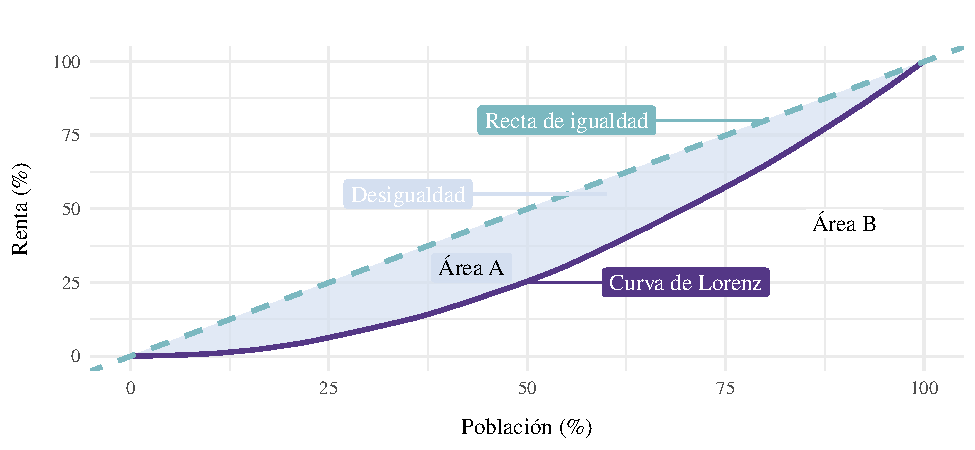
\includegraphics{Informe_files/figure-latex/Figura5-1} 

}

\caption{Índice de Gini en un caso hipotético}\label{fig:Figura5}
\end{figure}

Para comprender la lógica, se puede observar en la Figura 5 que el 50\%
de la población alcanza un 25\% del ingreso mientras que un 75\% de la
población llega a más del 50\% del ingreso, es decir, el ingreso que
logra el 50\% de la población lo alcanza el 25\% contiguo, lo cual
indica desigualdad ya que el ingreso no estaría equitativamente
distribuido.

Se propone incorporar el índice de Gini al cálculo del IDH como
\((1-\frac{GINI}{100})\) para que un país más desigual en términos
salariales tenga menos desarrollo.

\subsubsection{Modificación en el cálculo del
IDH}\label{modificaciuxf3n-en-el-cuxe1lculo-del-idh-1}

A continuación se presentan las distintas maneras de incorporar el
coeficiente de Gini al cálculo de la dimensión de nivel estándar de vida
decente analizadas.

\begin{enumerate}
\def\labelenumi{\arabic{enumi}.}
\tightlist
\item
  Se planteo multiplicar \(1-\frac{GINI}{100}\) por el PNB de cada país
  y luego convertir la métrica resultante en un índice. Para ello se
  consideró el cero natural del cálculo del índice de PNB y como
  objetivo aspiracional se tomó el valor máximo observado de la nueva
  variable calculada. De esta forma el cálculo es el siguiente:
\end{enumerate}

\[PNB_{Gini} = PNB * \left(1-\frac{GINI}{100}\right)\]

\[\text{Índice de dimensión}_\text{Ingreso}=\frac{\ln(PNB_{Gini})-\ln(100)}{\ln(\max(PNB_{Gini}))-\ln(100)}\]

\begin{figure}
\centering
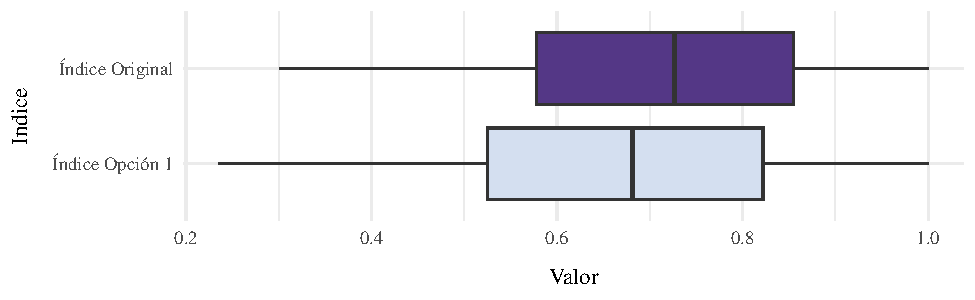
\includegraphics{Informe_files/figure-latex/Figura6-1.pdf}
\caption{Índice de PNB obtenido con la metodología original y la opción
1}
\end{figure}

Esta modificación del cálculo, en comparación con el original, devuelve
valores menores y cambian sus medidas descriptivas de posición, como la
mediana, lo cual da indicio de que la posición de los países podría
cambiar. Esto se puede observar en la Figura 6.

\begin{enumerate}
\def\labelenumi{\arabic{enumi}.}
\setcounter{enumi}{1}
\tightlist
\item
  Una segunda opción considerada fue calcular el índice de PNB y luego
  multiplicarlo por \(1-\frac{GINI}{100}\). Esta opción disminuía
  demasiado los valores de esta dimensión por lo que también se probó
  aplicarle la raíz \(1-\frac{GINI}{100}\), logrando que tenga menos
  peso esta penalización.
\end{enumerate}

\[\text{Índice de dimensión}_\text{Ingreso} = \text{Índice de PNB} \times \sqrt{1-\frac{GINI}{100}}\]

En la Figura 7 se puede observar el cambio abrupto mencionado al no
utilizar la raíz en la corrección y cómo la incorporación de la misma
diminuir esta penalización. De todas formas, el cambio con esta opción
continúa siendo abrupto en comparación con la opción 1.

\begin{figure}
\centering
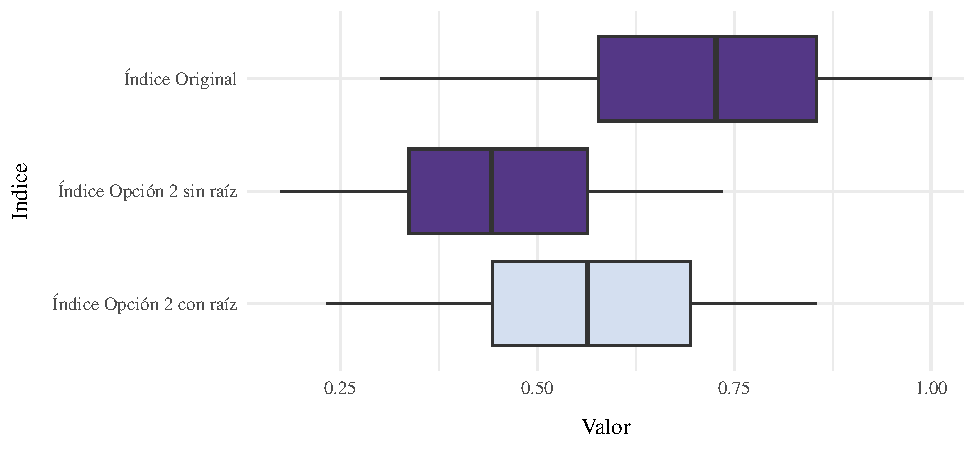
\includegraphics{Informe_files/figure-latex/Figura7-1.pdf}
\caption{Índice de PNB obtenido con la metodología original y los
diferentes enfoques de la opción 2}
\end{figure}

Después de analizar ambas opciones, se consideró mejor la multiplicación
del coeficiente de Gini previo al cálculo del índice, es decir la opción
1. Puesto que los valores de la segunda opción resultan ser
considerablemente menores. Además, otro factor importante es que se
intenta que los índices de cada dimensión puedan tomar un valor cercano
1 y esta alternativa no permite esta opción por la naturaleza de su
cálculo.

En el Cuadro 2 donde se muestran los 5 países con menor PNB ajustado por
Gini, puede visualizarse que hay una variación en el puesto de los
países al comparar el Índice Original y el Modificado. Los cambio con el
índice modificado generará una especie de penalización en elcálculo del
IDH a aquellos países que no reparten equitativamente sus ingresos.

\begin{table}[H]

\caption{\label{tab:unnamed-chunk-2}Resultados del Índice modificado}
\centering
\begin{tabular}[t]{c|c|c|c|c}
\hline
País & PNB & PNB ajustado Gini & Índice Original & Índice Modificado\\
\hline
South Sudan & 784.4744 & 438.5212 & 0.3111512 & 0.2353895\\
\hline
Burundi & 732.0426 & 449.4742 & 0.3007019 & 0.2393179\\
\hline
Democratic Republic of the Congo & 998.1225 & 577.9129 & 0.3475348 & 0.2793412\\
\hline
Mozambique & 1265.0711 & 626.2102 & 0.3833362 & 0.2921220\\
\hline
Yemen & 1165.0907 & 737.5024 & 0.3708998 & 0.3181704\\
\hline
\end{tabular}
\end{table}

\subsection{Una nueva rama para el IDH: Libertad, derechos políticos y
libertades
civiles}\label{una-nueva-rama-para-el-idh-libertad-derechos-poluxedticos-y-libertades-civiles}

\subsubsection{Debate}\label{debate-2}

A pesar de la importancia de las métricas económicas, índices de salud y
de educación, el IDH no considera un aspecto relevante del desarrollo
humano: la libertad. En esta sección se propone implementar este
concepto como una nueva dimensión, entendiendo como libertad al pleno
ejercicio de los derechos políticos y de las libertades civiles, bajo un
régimen libre, democrático y plural. La libertad permite a las personas
tomar decisiones sobre sus vidas, perseguir sus objetivos y contribuir a
la sociedad. La falta de ella puede obstaculizar el acceso a la
educación, la salud y otras oportunidades, perpetuando desigualdades.

Los mismos autores del IDH reconocieron, en el informe de desarollo
humano de 2010, que el cálculo no contaba con una ``medida cuantitativa
de la libertad humana''.

\subsubsection{Modificación en el cálculo del
IDH}\label{modificaciuxf3n-en-el-cuxe1lculo-del-idh-2}

Se propone un enfoque innovador que complemente a las dimensiones
existentes del IDH: salud, educación e ingreso per cápita. Al incorporar
la libertad, el IDH puede reflejar una imagen más completa del bienestar
de las naciones, teniendo en cuenta cuestiones sociales que no están
contempladas actualmente. Si bien la incorporación de la libertad como
nueva dimensión del desarrollo humano puede generar debates sobre su
naturaleza ideológica o subjetiva, se piensa que su inclusión es
necesaria para medir el progreso de una nación y el bienestar de sus
habitantes. Se busca implementar una metodología que cuantifique estas
problemáticas, mediante un índice que permita una evaluación integral y
completa de cada territorio, considerando sus particularidades.

Para su aplicación se toma el índice de libertad ``Freedom in the
World'', publicado por la organización Freedom House. La misma es una
ONG estadounidense fundada en 1941 con el fin de reunir políticos y al
público del país en torno a la lucha contra la Alemania nazi y para
crear conciencia sobre la amenaza facista a la seguridad y a los valores
estadounidenses. En las décadas posteriores, Freedom House se
estableció, a través de sus programas e investigaciones, como la
principal organización estadounidense dedicada al apoyo y la defensa de
la democracia y la libertad en todo el mundo. A pesar de que esta visión
tiene un enfoque puramente occidental, se considera su inclusión dado
que es una medida abarcativa de esta problemática.

Este puntaje se centra en dos ejes principales, derechos políticos y
libertades civiles, y tiene en cuenta los siguientes factores:

\paragraph{Derechos políticos}\label{derechos-poluxedticos}

\begin{itemize}
\item
  \textbf{Proceso electoral}: elecciones que cumplen con estándares
  democráticos reconocidos, transparentes, libres, universales, etc.
\item
  \textbf{Pluralismo y participación política}: ausencia de obstáculos o
  restricciones discriminatorias, intimidación, violencia contra
  miembros o líderes políticos; oportunidad realista de alternancia en
  el poder; elecciones libres de poderes externos; diversos segmentos de
  la población (incluidos grupos étnicos, raciales, religiosos, de
  género, LGBT+ y otros relevantes) tienen plenos derechos políticos,
  oportunidades electorales, etc.
\item
  \textbf{Funcionamiento del gobierno}: se evalúa si los representantes
  elegidos libremente pueden determinar las políticas del gobierno sin
  interferencia de actores estatales y no estatales en la adopción y
  ejecución de políticas, así como el control de las fuerzas armadas y
  la influencia extranjera sobre las decisiones gubernamentales; la
  existencia de mecanismos efectivos contra la corrupción y la
  transparencia de las decisiones tomadas.
\end{itemize}

\paragraph{Libertades civiles}\label{libertades-civiles}

\begin{itemize}
\item
  \textbf{Libertad de expresión y creencias}: medios de comunicación
  libres e independientes; libertad de culto en público y privado;
  libertad académica, educación libre de adoctrinamiento político;
  libertad de expresión sin represalias.
\item
  \textbf{Derecho de asociación y organización}: se evalúa si las
  protestas pacíficas están prohibidas o restringidas; si existe libre
  funcionamiento de las ONG; libertad para los sindicatos y asociaciones
  laborales sin interferencia del gobierno, y sin presiones de parte de
  los sindicatos hacia los trabajadores; derecho de huelga.
\item
  \textbf{Estado de derecho}: poder judicial independiente; asignación y
  destitución de jueces de manera justa e imparcial; prevalece el debido
  proceso, defendiendo los derechos del acusado y de la población
  carcelaria; protección contra el uso ilegítimo de la fuerza física de
  parte de las fuerzas policiales; igualdad ante la ley y ausencia de
  discriminación legal o de facto para grupos étnicos, raciales,
  religiosos, de género, LGBT+ y otros.
\item
  \textbf{Autonomía personal y derechos individuales}: libertad de
  circulación; derecho de propiedad; igualdad de oportunidades, derechos
  laborales y movilidad social; tiene en consideración la existencia de
  violencia doméstica, mutilación genital femenina, abuso sexual y
  violación, con justicia efectiva para los perpetradores; si el
  gobierno impone restricciones sobre anticonceptivos o aborto; si se
  controla la vestimenta, la expresión de género o prohibe el matrimonio
  igualitario; si interviene en la elección de parejas o relaciones
  personales mediante leyes restrictivas, si garantiza igualdad en
  procedimientos de divorcio y custodia, y si protege las libertades
  personales frente a instituciones privadas o grupos sociales.
\item
  \textbf{Derechos políticos discrecionales}: indaga si el gobierno o
  una potencia ocupante están alterando deliberadamente la composición
  étnica de un país o territorio para destruir una cultura o inclinar el
  equilibrio político a favor de otro grupo.
\end{itemize}

\subsubsection{Cálculo del nuevo
índice}\label{cuxe1lculo-del-nuevo-uxedndice}

Esta dimensión está formada por 25 indicadores relacionados a los
factores descritos anteriormente. Los puntajes de cada uno de ellos son
definidos por un equipo de analistas internos y externos de la
organización y de asesores expertos de comunidades académicas y de
derechos humanos. Ellos usan una gran variedad de recursos que incluyen
artículos de noticias, análisis académicos, reportes de ONGs e
investigaciones del campo. El puntaje se determina basándose en las
condiciones o eventos dentro del país en un año determinado. El producto
final se define a partir del consenso de los analistas quienes proponen
puntajes que son discutidos y defendidos a través de una serie de
encuentros del equipo nombrado dentro de Freedom House.

Cada uno de los indicadores toma un valor discreto de 0 a 4, formando un
puntaje para cada país y territorio. La pregunta relacionada con los
derechos políticos discrecionales penaliza dicho puntaje obtenido con el
resto de las preguntas, restando hasta 4 puntos. De esto surge un
puntaje, en principio de 0 a 100 por país, que es dividido por 100 e
incorporado al IDH como una nueva rama independiente de las ya
existentes, con el mismo peso.

Para su incorporación al IDH propuesto, surge el debate entre incorporar
a todas las preguntas o incluir sólo las referidas a las libertades
civiles. De esta manera, se dejaría de lado a las que se refieren al
tipo de gobierno adoptado de cada territorio por las diferencias
culturales que existen entre las distintas regiones del mundo, que
pueden influir en los sistemas de gobierno adoptados. Al comparar el
puntaje recibido únicamente referido a derechos políticos con el puntaje
de libertades civiles se obtiene una alta correlación (0.96), por lo que
muy posiblemente se llegue a los mismos resultados. Además de eso, en
este informe se considera a los valores democráticos y al Estado de
derecho como factores positivos para el pleno desarrollo humano y para
posibilitar el ejercicio del bienestar del mismo, por lo tanto, se
decide incorporar a la totalidad de las preguntas en este indicador.

A pesar de que este índice posee cierto grado de subjetividad con
tendencia a la ideología estadounidense, este fue el resultado de una
búsqueda profunda de una medida que logre cuantificar la presente
dimensión y que sea comparable en los distintos países. Lo ideal sería
poder formar un índice con un enfoque más objetivo considerando
indicadores que demuestren concretamente las libertades de una
población. Sin embargo, dada la falta de variables que logren abarcar
esta amplia problemática y que estén cuantificadas en variedad de
países, sumado a la complejidad que conllevaría formar este índice desde
cero, este acercamiento es una buena aproximación de lo que se considera
como un ideal de un país libre y democrático. Queda propuesto el
análisis de esta nueva dimensión para una futura investigación.

\pagebreak

\section{IDH modificado: implementación de las
propuestas}\label{idh-modificado-implementaciuxf3n-de-las-propuestas}

Los índices elegidos resultan:

\begin{itemize}
\tightlist
\item
  Índice de salud: reemplazar la esperanza de vida al nacer por la
  esperanza de vida saludable al nacer.
\end{itemize}

\[\text{Índice de salud*} = \frac{\text{esp. vida saludable}-17.41872}{74.75077-17.41872}\]

\begin{itemize}
\tightlist
\item
  Índice económico: multiplicar \(1-\frac{GINI}{100}\) por el PNB de
  cada país y luego convertir la métrica resultante en un índice.
\end{itemize}

\[PNB_{Gini} = PNB \times \left(1-\frac{GINI}{100}\right)\]

\[\text{Índice del ingreso*}=\frac{\ln(PNB_{Gini})-\ln(100)}{\ln(53377.0398)-\ln(100)}\]

\begin{itemize}
\item
  Índice de Conocimiento: permanece sin modificaciones.
\item
  Índice de Libertad: Se toma en consideración a la totalidad de las
  preguntas realizadas en el índice de libertad ``Freedom in the World''
  del año 2019 (ACLARAR EL AÑO TAMBIEN ARRIBA QUE NO ESTA), publicado
  por la organización Freedom House.
\end{itemize}

\[\text{Índice de libertad } = Puntaje/100\]

Una vez obtenido los índices de cada dimensión, se decide calcular dos
nuevos índices de Desarrollo Humano, uno sin incluir a la nueva rama de
Libertad y otro que la incluya. Se toma esta decisión para observar cómo
las modificaciones a las ramas ya existentes del IDH alteran los
resultados y, por otro lado, evaluar si la inclusión de esta nueva
dimensión cambia las conclusiones, sugiriendo que hasta ahora podría
haberse estado ignorando un aspecto crucial del desarrollo humano.

Los nuevos IDH modificados se calculan mediante una media geométrica de
los respectivos índices obtenidos, de igual forma que en el IDH
original.

Índice sin Libertad:
\[IDH_\text{sin libertad} = (\text{Índice de salud*}\times\text{Índice de educación}\times\text{Índice del ingreso*})^{1/3}\]

Índice con Libertad:
\[IDH_\text{sin libertad} = (\text{Índice de salud*}\times\text{Índice de educación}\times\text{Índice del ingreso*}\times\text{Índice de libertad})^{1/3}\]

Cabe aclarar que los países que presentan al menos un valor faltante de
las variables consideradas en el estudio fueron descartadas del mismo.
Al recolectar todos los datos para el año 2019 finalmente se cuenta con
151 países de un total de 195 para los cuales fue calculado el IDH
original en el Informe de Desarrollo Humano del mismo año.

\section{Resultados}\label{resultados}

Una vez determinadas todas las modificaciones a las dimensiones, se
procede a aplicarlas al cálculo de los IDH modificados mencionados en la
sección anterior. Se denomina \texttt{IDH2} al índice con modificaciones
sin Libertad e \texttt{IDH3} al que sí tiene incluído la nueva
dimensión.

Los resultados obtenidos se muestran en la siguiente tabla, donde los
países se encuentran ordenados según el IDH original y se muestran los 3
índices, con una escala de color y sus respectivos ranqueos y cambios de
puestos.

\pagebreak

Tabla 1: Índices de Desarrollo Humano por país

\begin{center}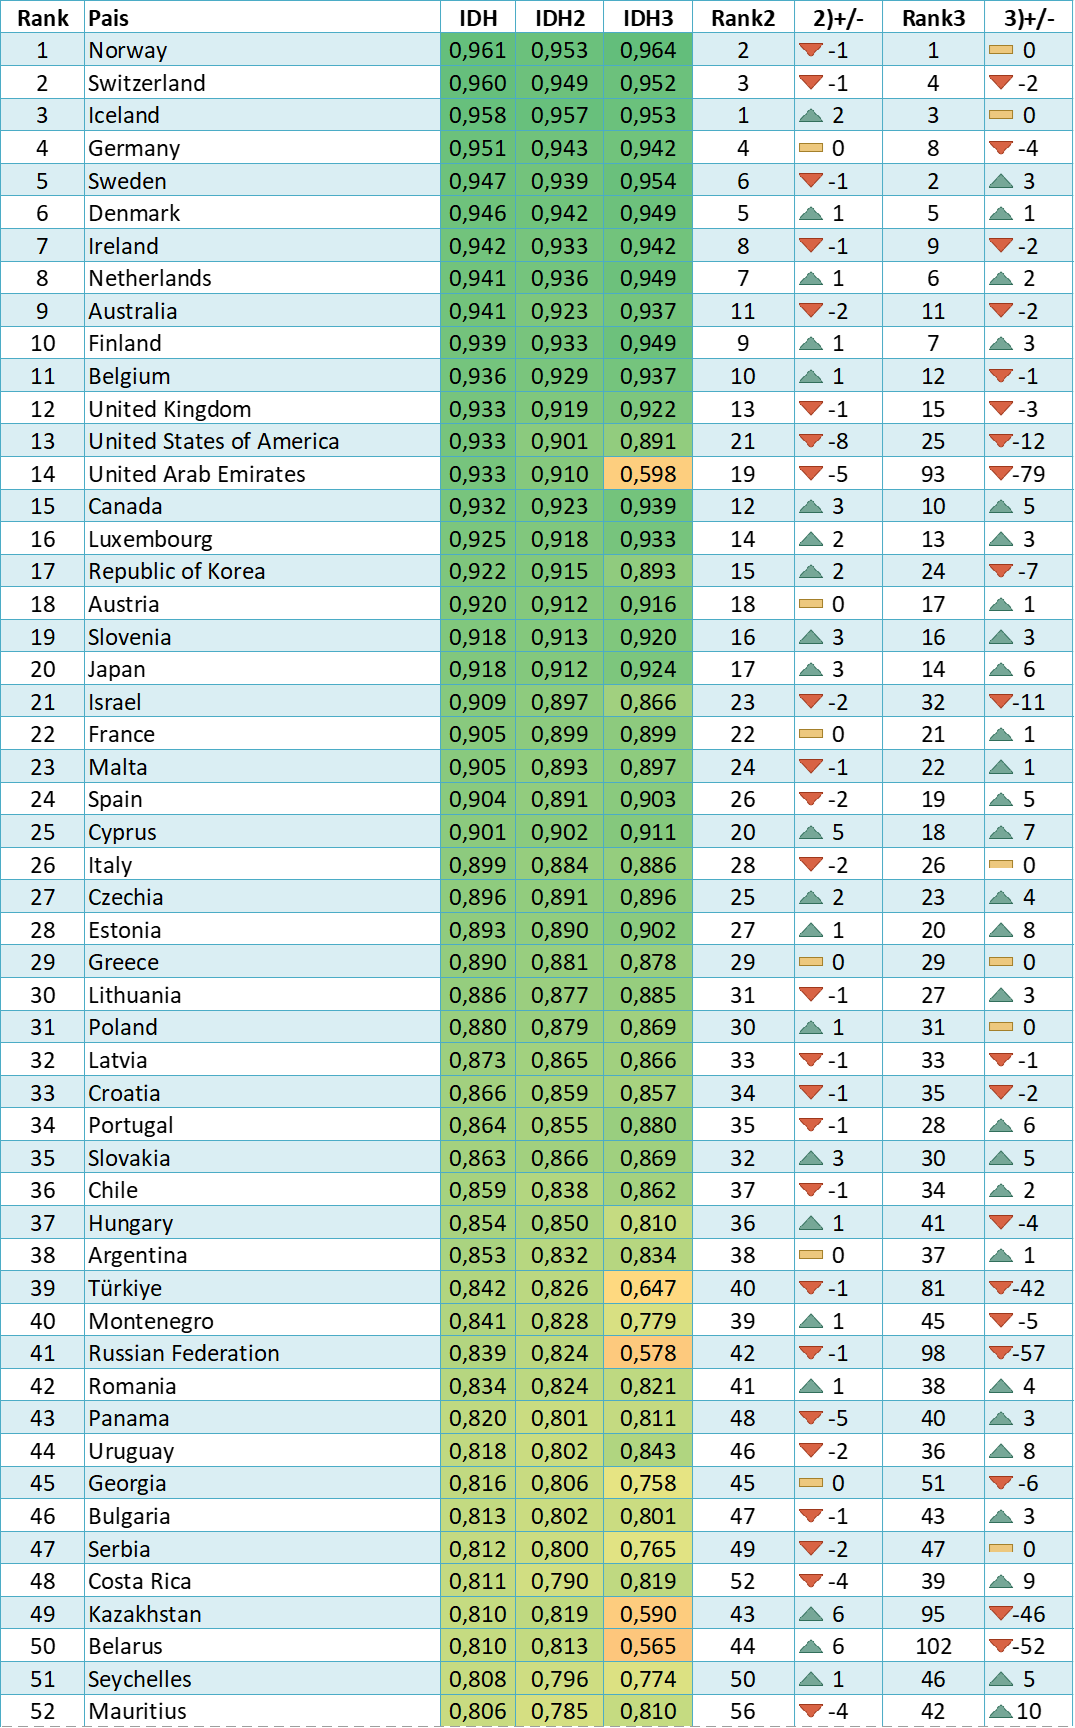
\includegraphics[width=0.75\linewidth]{Resultados/Tabla_IDH1} \end{center}

\pagebreak

\begin{center}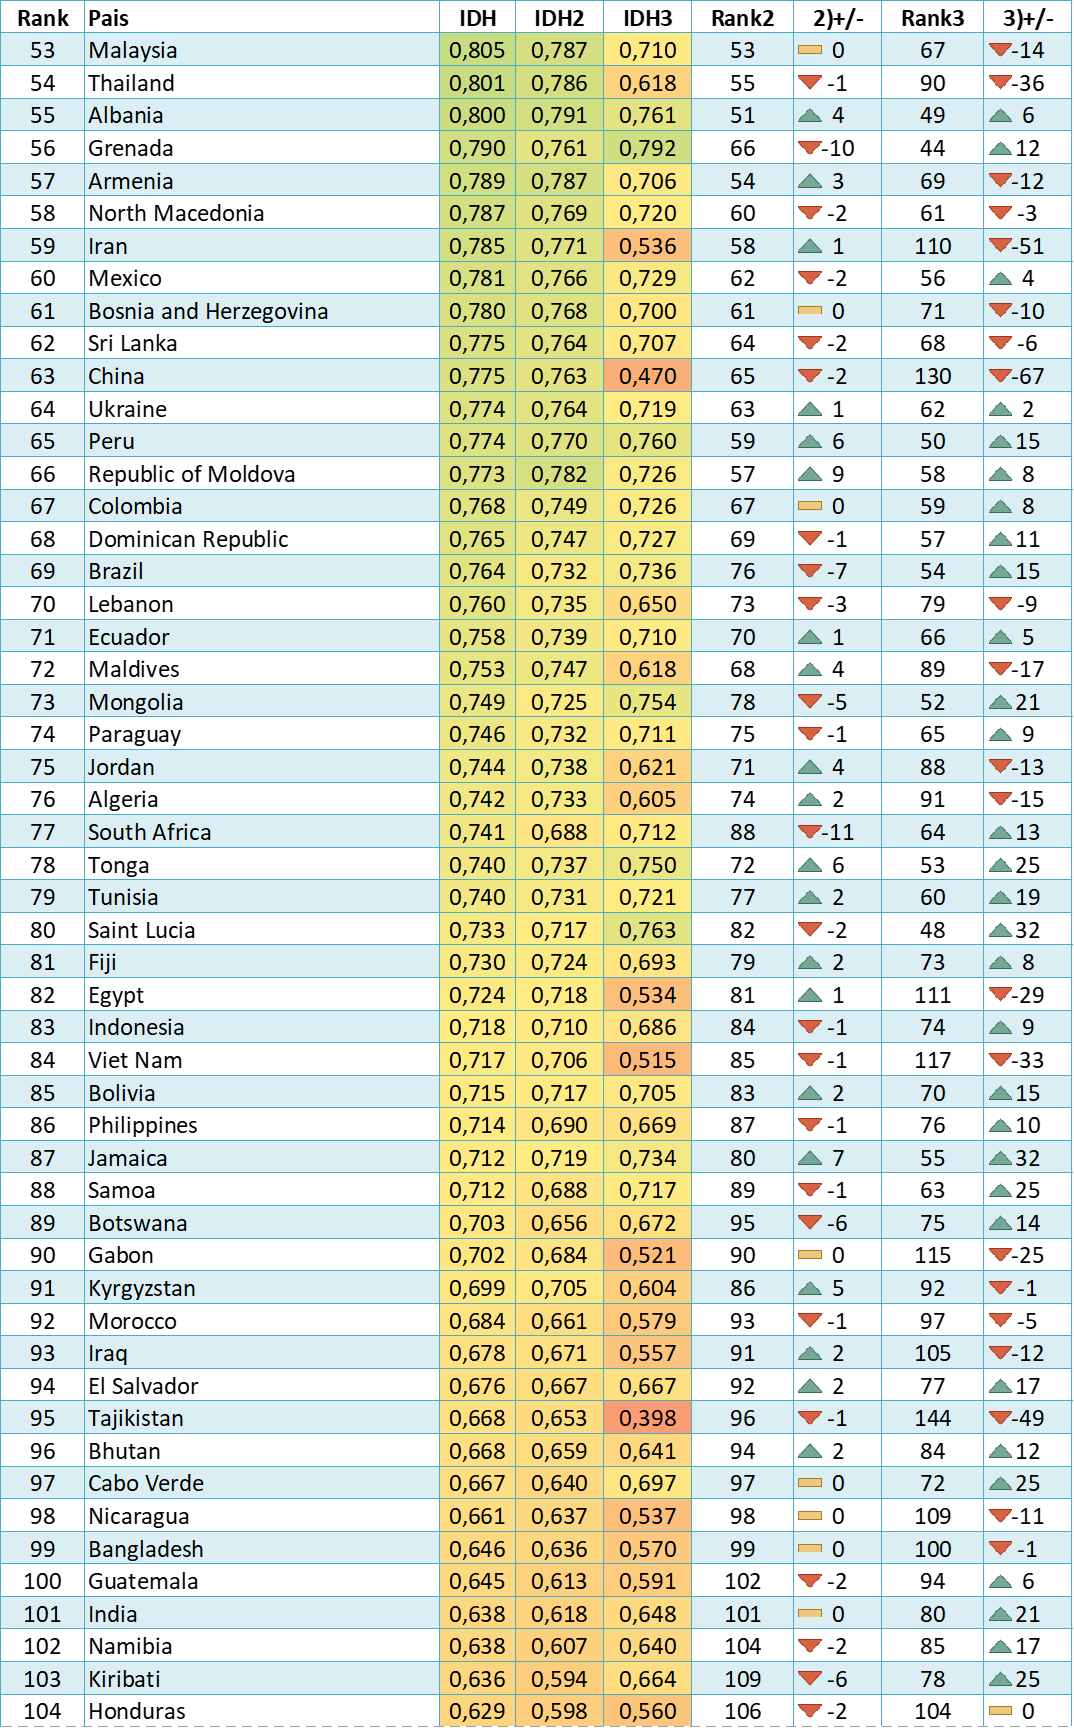
\includegraphics[width=14.92in]{Resultados/Tabla_IDH2} \end{center}
\pagebreak

\begin{center}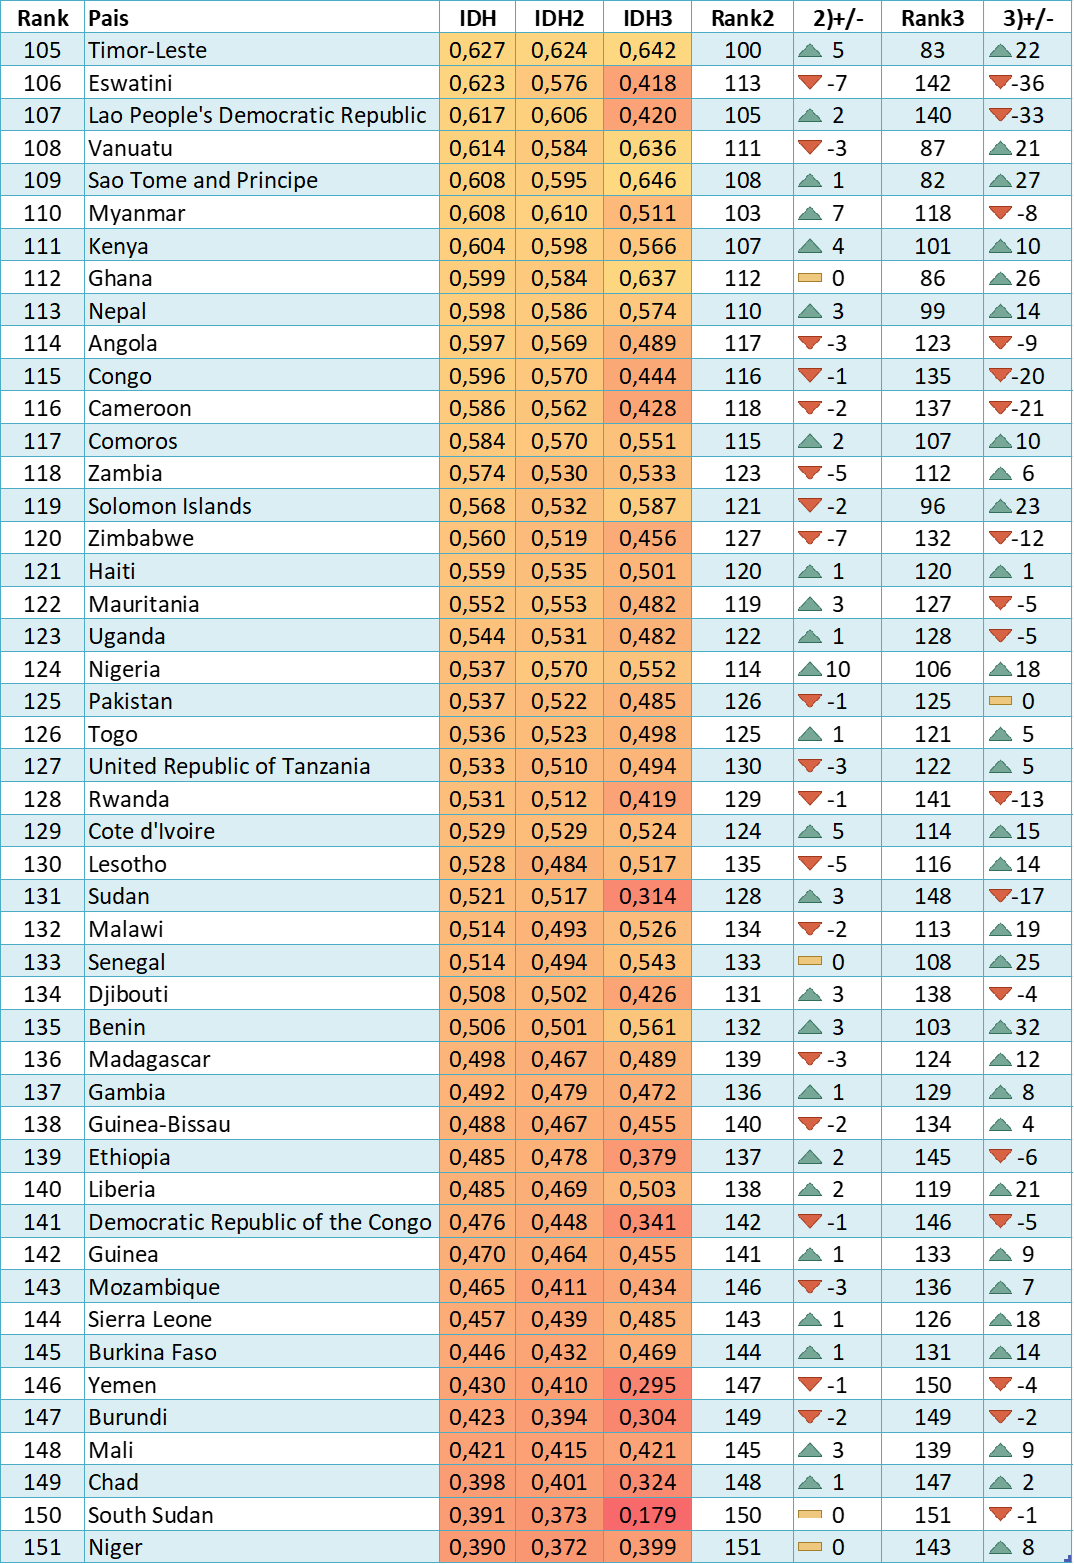
\includegraphics[width=14.92in]{Resultados/Tabla_IDH3} \end{center}

\pagebreak

La escala de color es de gran ayuda para facilitar la visualización de
las variaciones en los países. Por ejemplo, en la parte superior del
ranking, destacan países como Emiratos Árabes Unidos, donde se observa
claramente cómo la incorporación de la dimensión Libertad afecta en gran
medida su puntaje. Por otro lado, países como Costa Rica, Uruguay, Chile
y España suben su puntaje al agregar esta dimensión.

En el Anexo se encuentran las tablas con los países ordenados según
estas nuevas propuestas del IDH.

Luego de calcular y analizar los puntajes obtenidos, es posible realizar
una comparación de los índices junto con el desempeño de determinados
países respecto a estos.

Además se muestran mapas con los países coloreados según una escala
continua del IDH.

\begin{figure}

{\centering 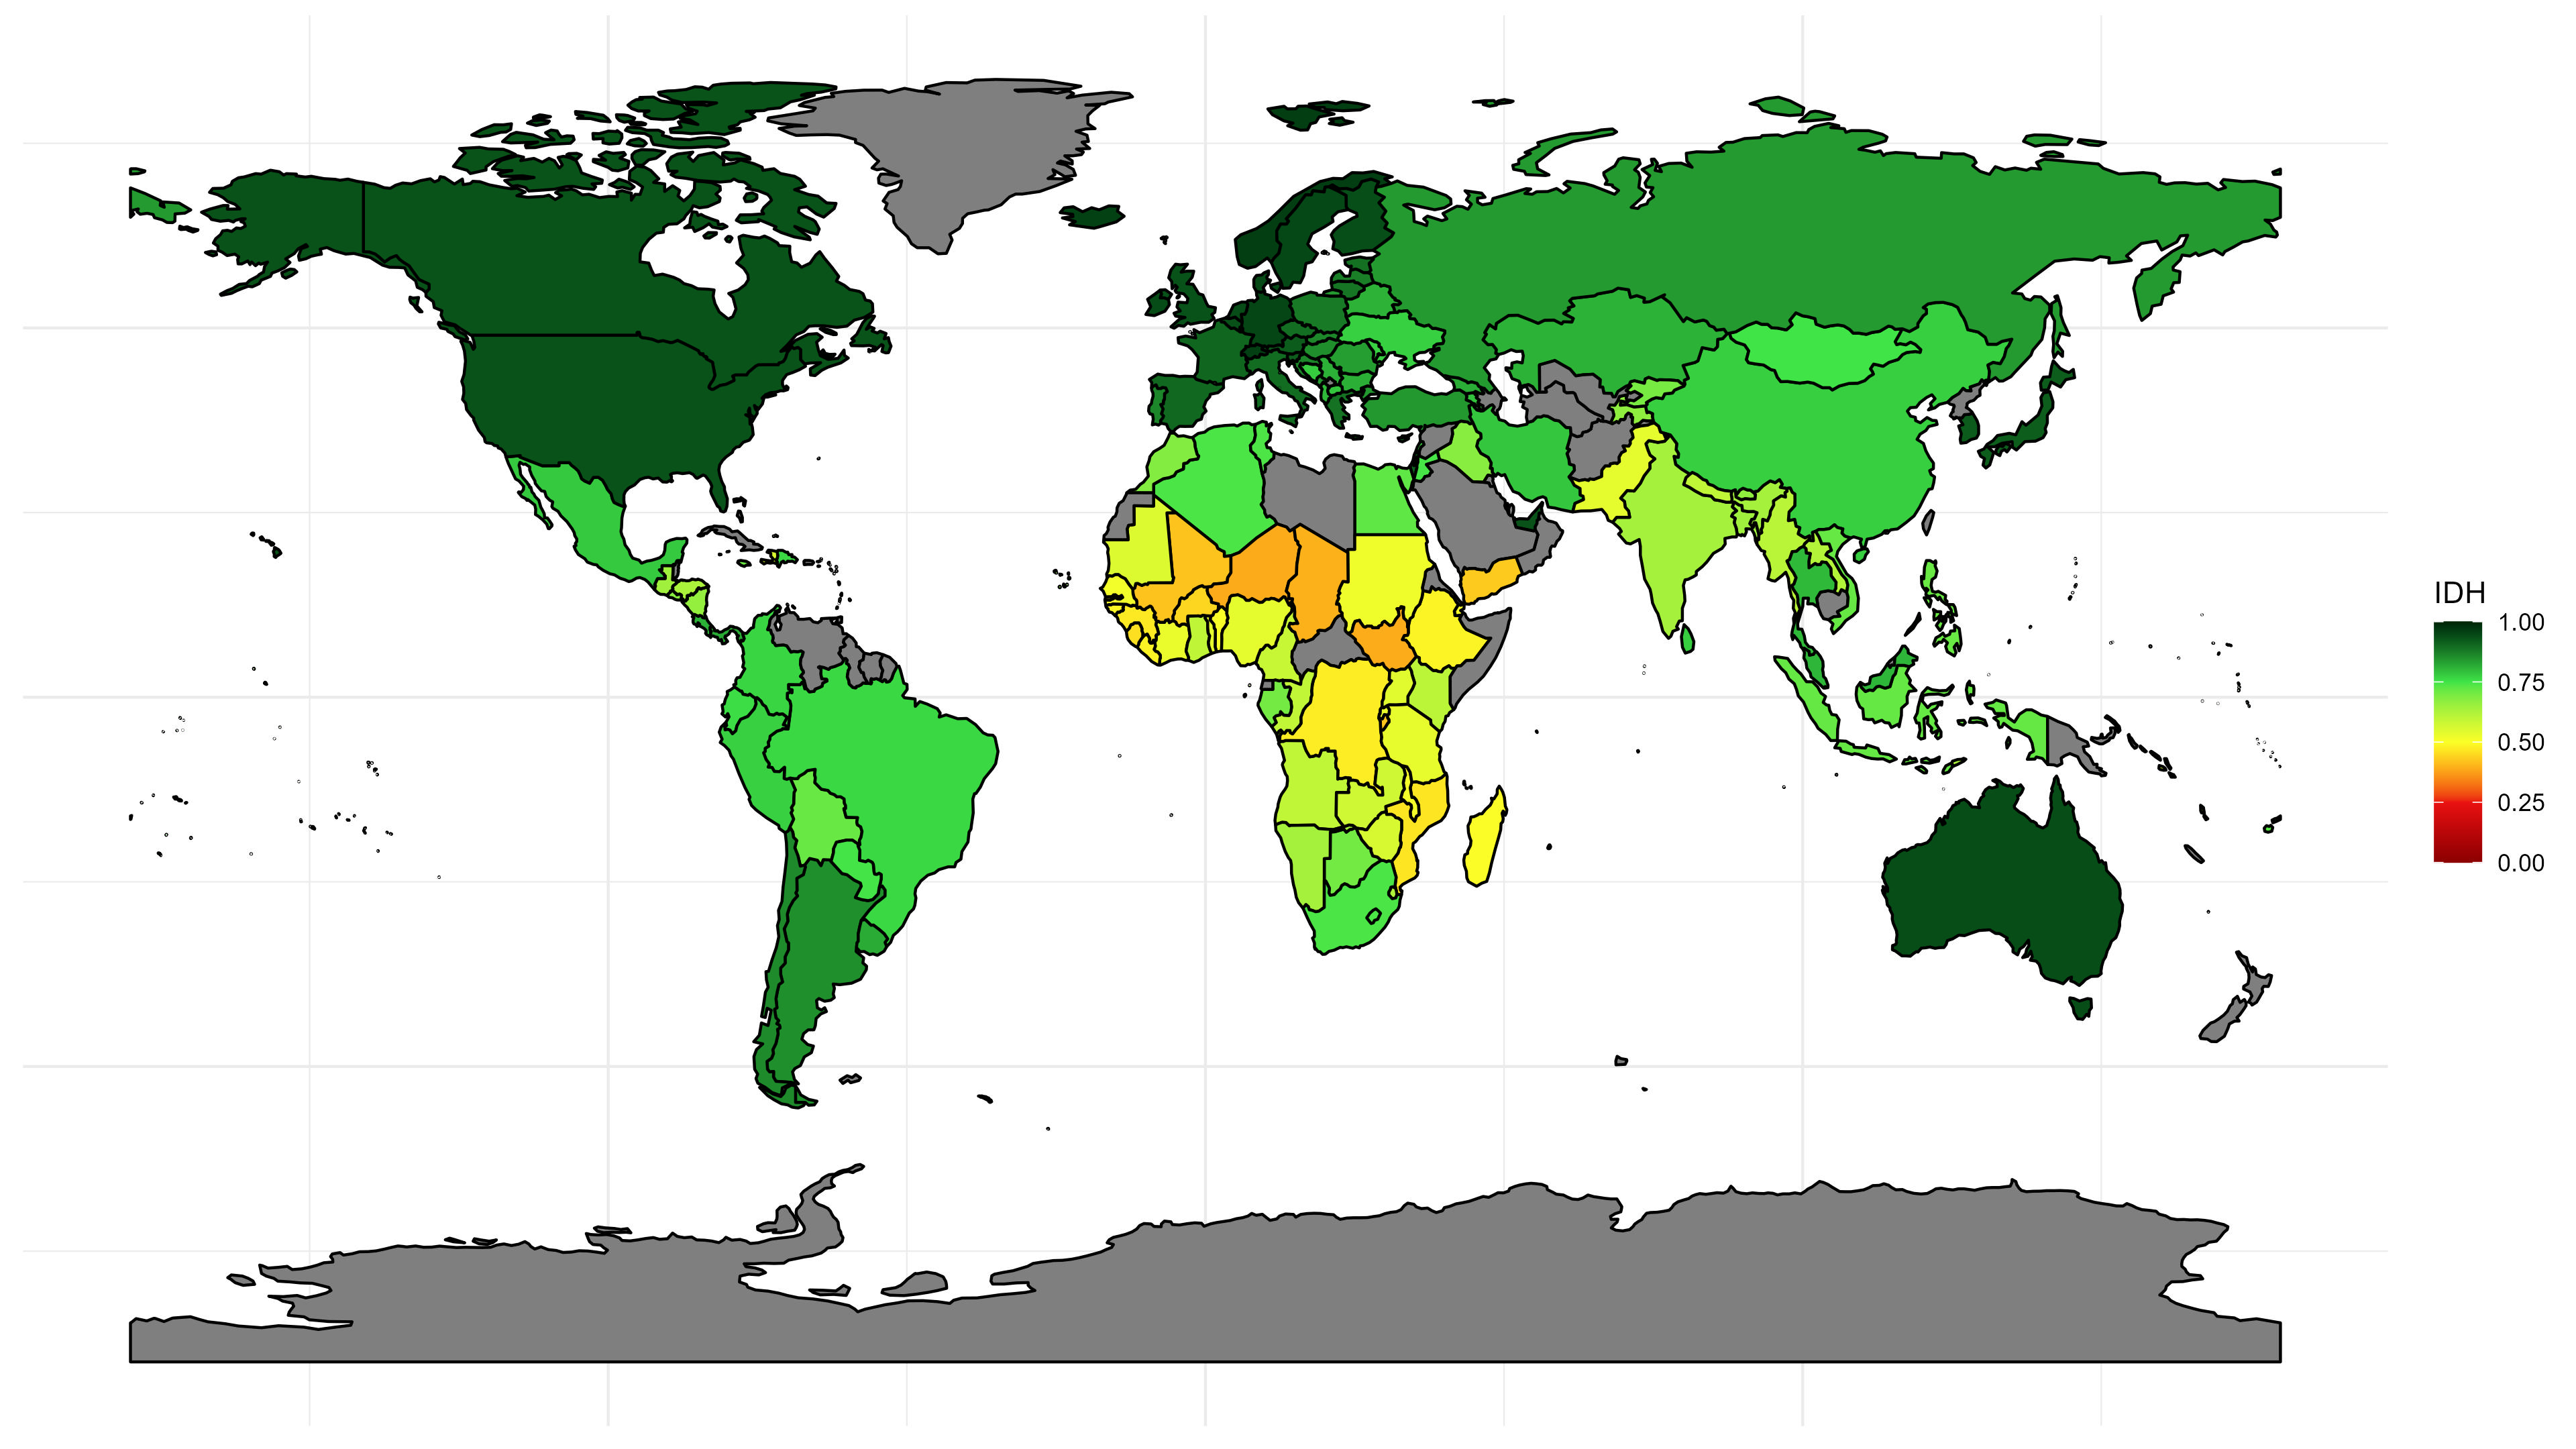
\includegraphics[width=1\linewidth]{Resultados/mapa_IDH1} 

}

\caption{Índice de Desarrollo Humano original por país}\label{fig:mapa1}
\end{figure}

Inicialmente, en cuanto al IDH original, se puede observar que en
América la mayoría de los países toman valores altos de desarrollo
humano, principalmente Estados Unidos, Canadá y el Cono Sur. Europa
también toma valores altos de este índice en casi todos sus países,
siendo el continente con más países con alto grado de desarrollo humano.
En Asia, a pesar de que la gran mayoría tome valores altos destacan
principalmente Japón y Corea del Sur y también se encuentran países que
toman valores intermedios. En Oceanía, se tiene únicamente información
sobre Australia el cual toma un valor alto del idh. Por último, África
es el continente donde hay más variabilidad del índice de idh,
presentando valores bajos, medios y altos.

\begin{figure}

{\centering 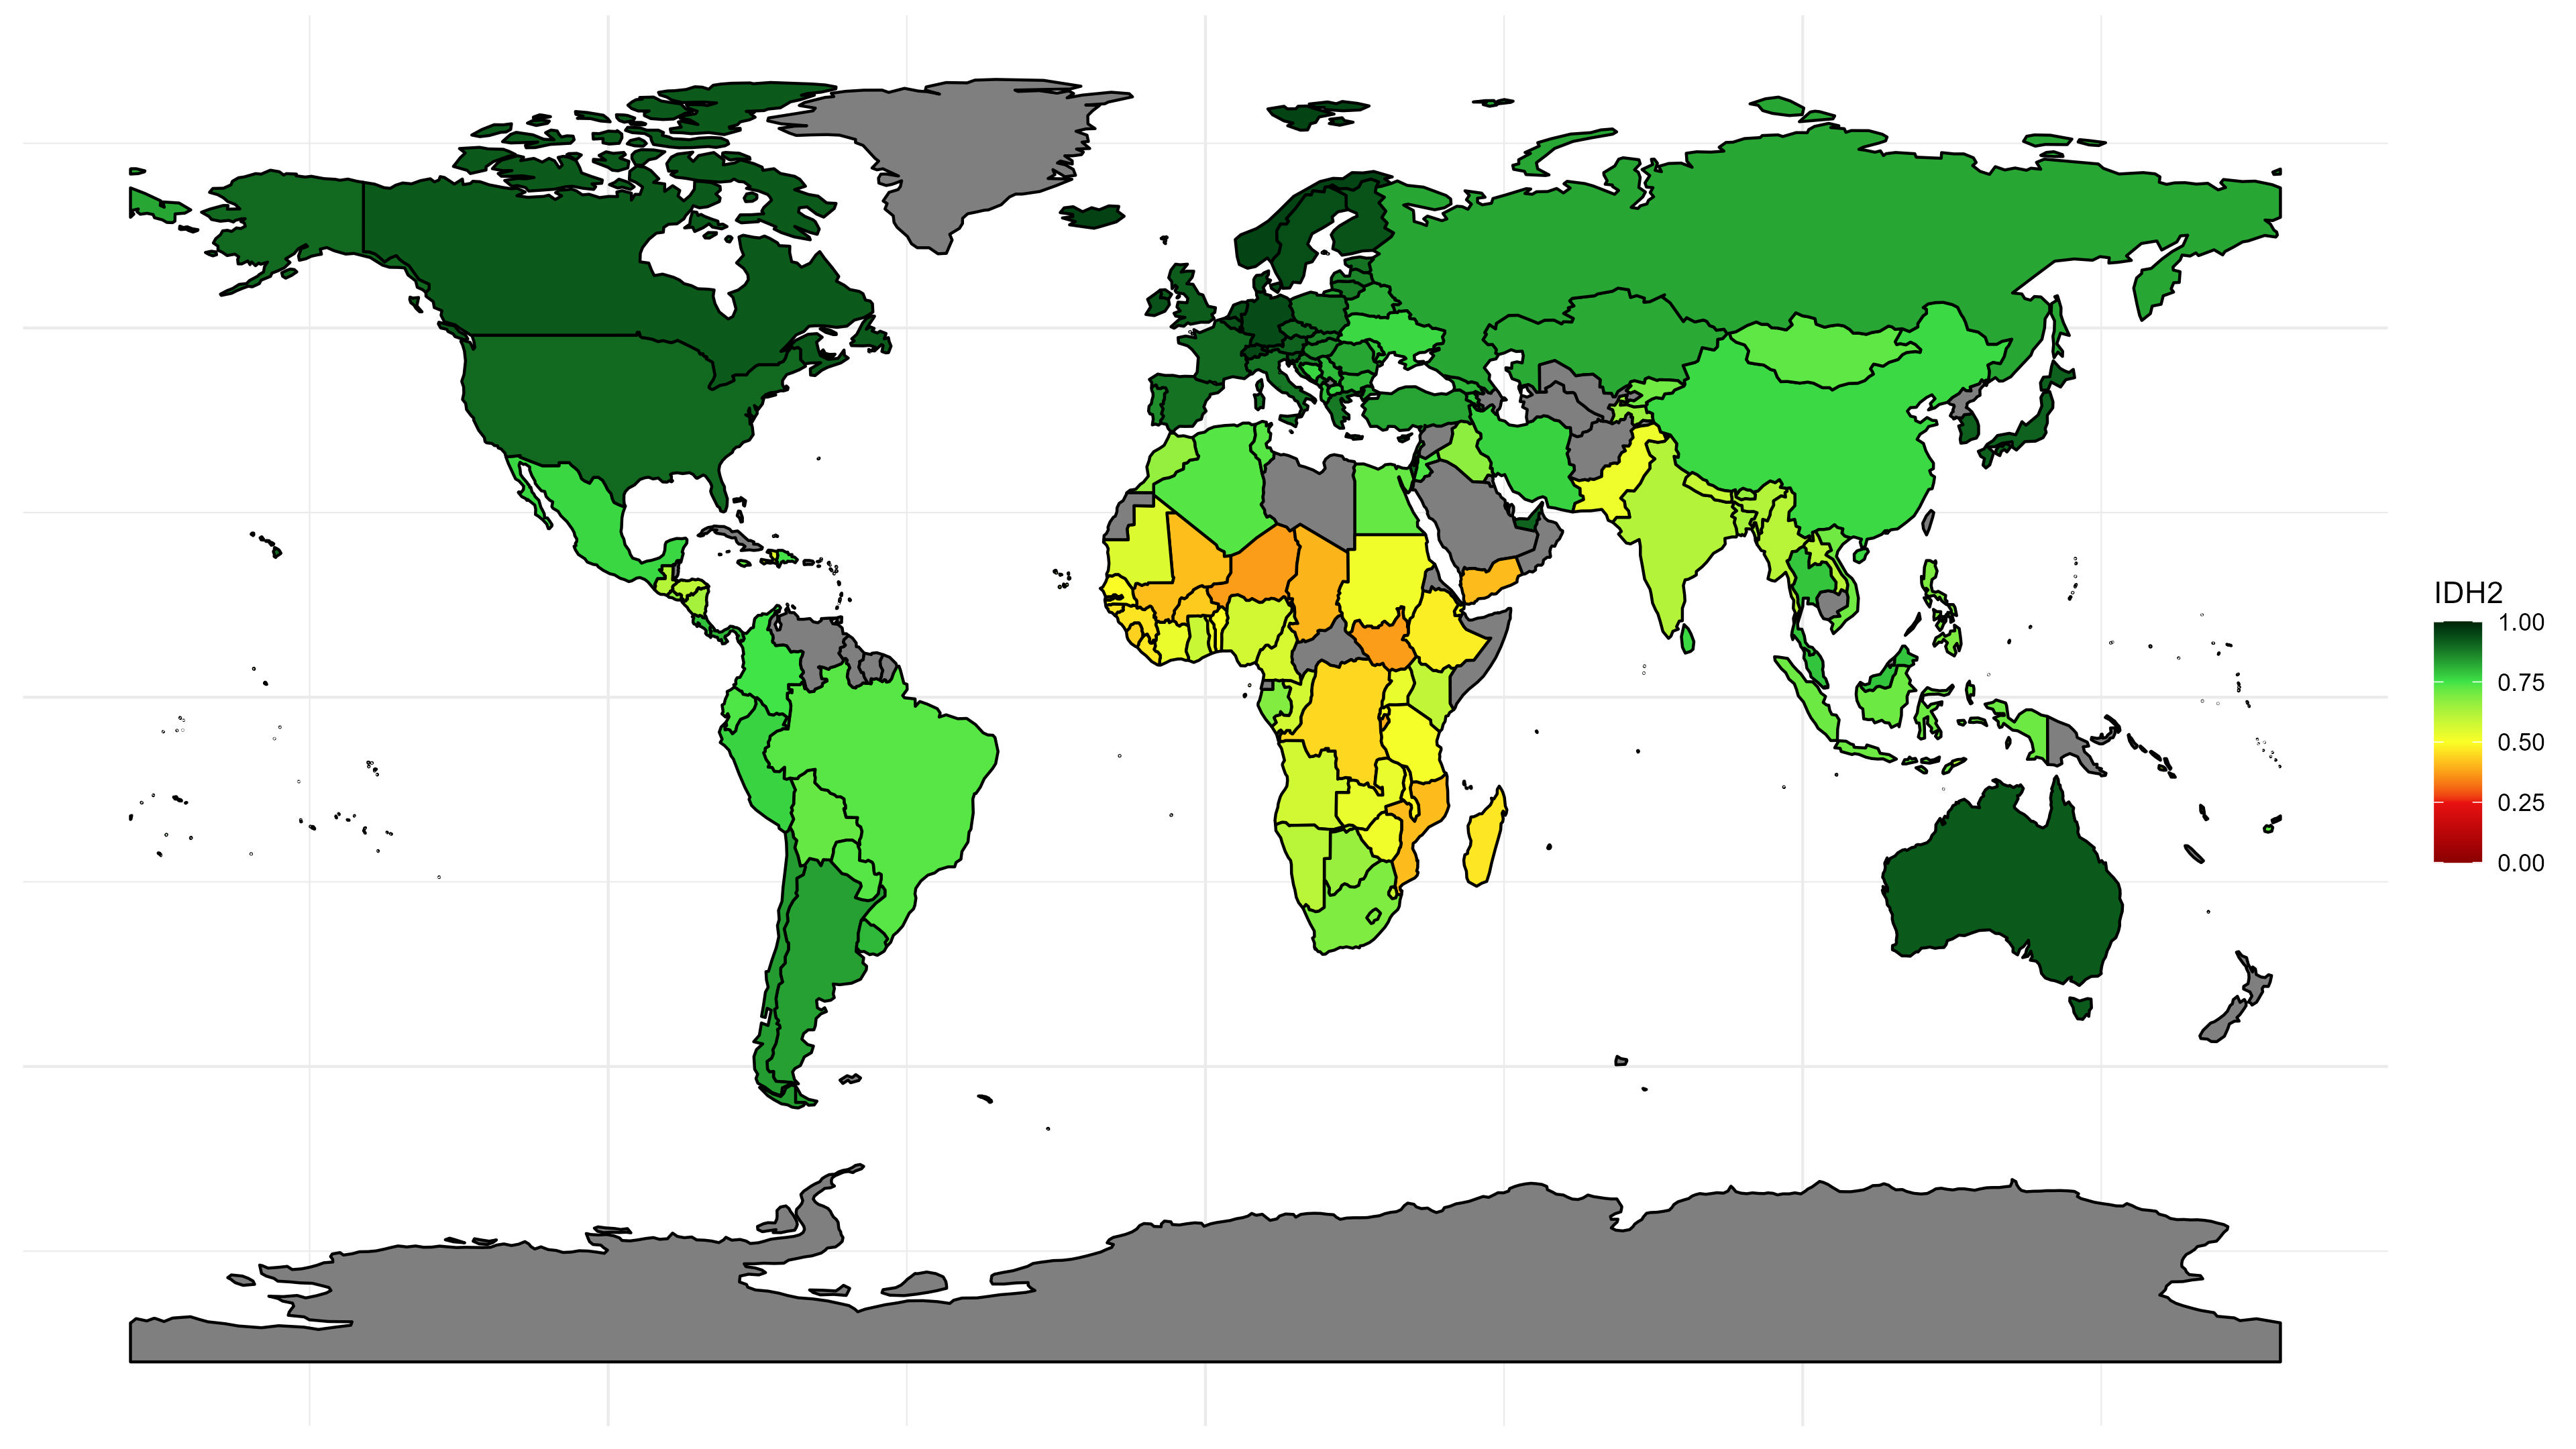
\includegraphics[width=1\linewidth]{Resultados/mapa_IDH2} 

}

\caption{Índice de Desarrollo Humano modificado sin Libertad por país}\label{fig:mapa2}
\end{figure}

Al calcular el IDH modificado sin considerar la dimensión de libertad,
no se observa una diferencia muy grande en cuanto a los valores de IDH
de cada país. Se puede notar una leve disminución general de este índice
en casi todos los países del mundo.

\begin{figure}

{\centering 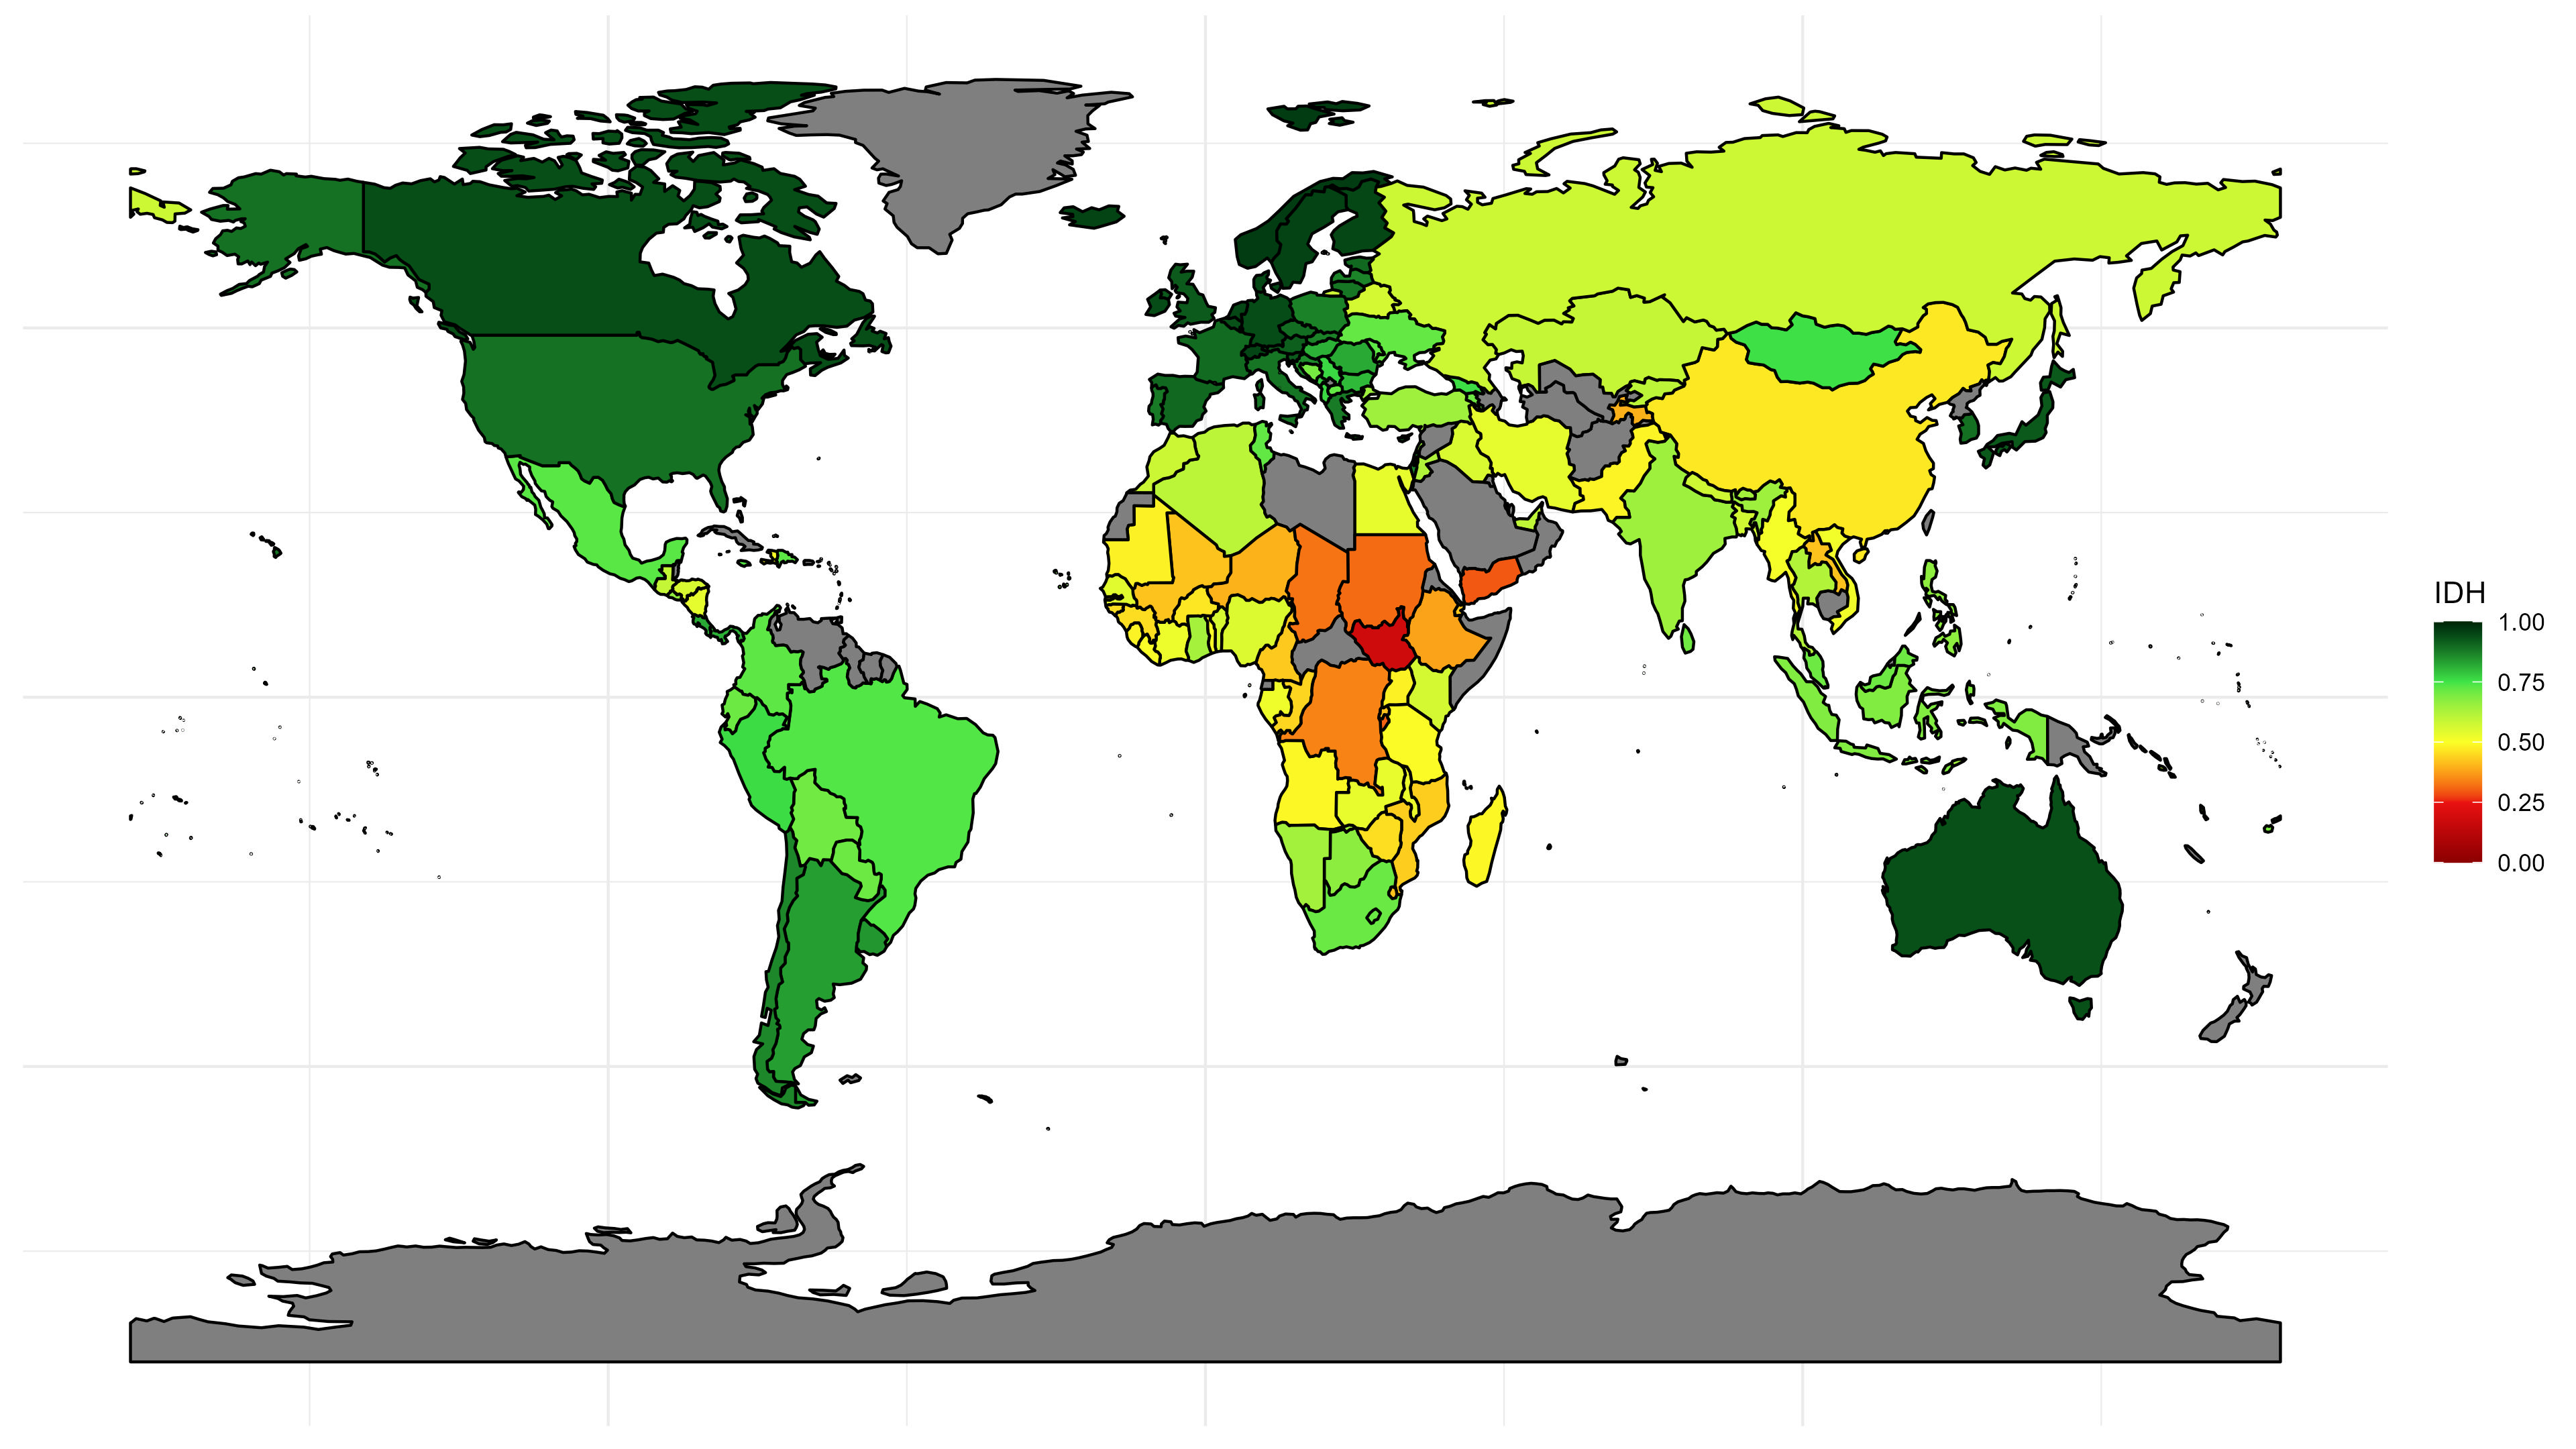
\includegraphics[width=1\linewidth]{Resultados/mapa_IDH3} 

}

\caption{Índice de Desarrollo Humano modificado con Libertad por país}\label{fig:mapa3}
\end{figure}

Por el contrario, al comparar el índice de desarrollo humano que incluye
la dimensión de libertad con el original se visualizan cambios
sustanciales. En América hay ciertos países que se aprecia una leve o
moderada disminución del IDH, principalmente países centroamericanos y
Estados Unidos. En Europa se mantienen valores altos para la mayoría de
los países, excepto para Rusia y Bielorusia, que bajan notablemente. En
Asia parece haber una importante disminución general de los puntajes,
excepto para países como Corea del Sur, Japón, India e Indonesia. En
África se observa algo similar que en Asia y se destaca a Sudán del Sur
por su muy bajo puntaje.

La dimensión de Libertad parece afectar principalmente en las regiones
africanas y asiáticas. Podría decirse que el mundo no occidental fue
altamente penalizado por posibles cuestiones culturales, principalmente
por presentar discrepancias con los pilares ideológicos estadounidenses,
que responden a un pensamiento occidental en materia política y social,
en los cuales se basa el índice de Libertad implementado.

\subsection{Análisis comparativo entre los
índices.}\label{anuxe1lisis-comparativo-entre-los-uxedndices.}

Se calcula la correlación entre los valores de los índices y el de los
puestos. Estos se muestran en la siguiente tabla

\begin{itemize}
\item
  Rankear los países con IDH modificado y comparar (2 gráficos países
  colores)
\item
  Corr entre los IDH y el/los modificados
\item
  Resulta diferente o no al IDH ventajas y desventajas
\item
  Idea mirando las tablas del informe del idh compara la clasificación
  de IDH con IDH modif por desigualdad viendo la diferencia. Ver si se
  podría y valdría la pena hacer lo mismo con el nuestro
\end{itemize}

\section{Cosas que quedan propuestas}\label{cosas-que-quedan-propuestas}

\section{Conclusión}\label{conclusiuxf3n}

\section{Categorías según desarrollo
humano}\label{categoruxedas-seguxfan-desarrollo-humano}

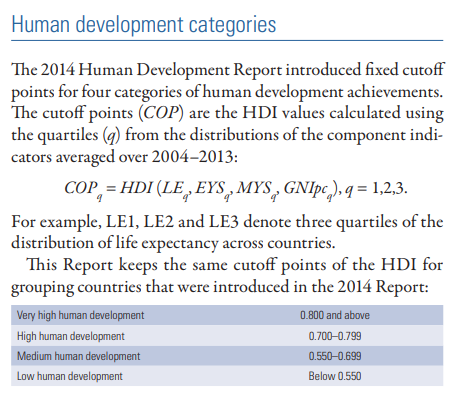
\includegraphics{agregar1.png}

Aggregate HDI values for country groups (by human development category,
region and the like) are calculated by applying the HDI formula to the
weighted group averages of component indicators. Life expectancy and GNI
per capita are weighted by total population, expected years of schooling
is weighted by population ages 5--24 and mean years of schooling is
weighted by population ages 25 and older.

\pagebreak

\section{Referencias}\label{referencias}

\subsection{Origen de los datos}\label{origen-de-los-datos}

Los datos obtenidos corresponden al año 2019. Se selecciona dicho año
por ser el más reciente previo a la pandemia de COVID-19, con el fin de
evitar posibles valores atípicos o cambios abruptos en determinados
países. La pandemia desarrollada en 2020 puede haber afectado el Índice
de Desarrollo Humano de los países, reduciendo la esperanza de vida
debido a la mortalidad, interrumpiendo la educación por el cierre de
escuelas y exacerbando las diferencias por el acceso desigual a la
virtualidad. Además, la recesión económica aumentó el desempleo y la
pobreza, afectando especialmente a los trabajadores informales y
amplificando las desigualdades preexistentes, impactando negativamente
los componentes clave del IDH en muchos países.

La base de datos fue armada en torno al Metadata original de las
Naciones Unidas, en la oficina de Reportes de Desarrollo Humano. De aquí
se obtiene toda la información oficial del IDH. En la base se tienen
todos los componentes del índice desde 1990 hasta el 2022. Para el
presente trabajo se tomaron los datos del año 2019. También desde el
mismo sitio se puede descargar cada uno de los informes, notas técnicas,
metodología, modificaciones del índice y otras publicaciones.

En la base final se tiene de esta fuente las siguientes variables:

\begin{itemize}
\item
  La esperanza de vida
\item
  Años de escolaridad esperados
\item
  Años de escolaridad promedio
\item
  Ingreso Nacional Bruto ajustado por paridad de poder adquisitivo
  (constante 2011)
\item
  El Índice de Desarrollo Humano original
\end{itemize}

Con estos datos se logró replicar el índice original, lo cual habla de
que se entendió la metodología utilizada, y se logró reproducir los
resultados oficiales. Por otro lado, los datos de las modificaciones
fueron importados de distintas fuentes.

Para empezar, los datos de esperanza de salud fueron obtenidos desde la
página de la Organización Mundial de la Salud. Este es un indicador
calculado por dicho organismo, que se implementa en la dimensión
modificada. Sus últimas actualizaciones fueron realizadas en el año
2020, tomando la esperanza de salud para el 2019.

La información del índice de Gini se obtuvo de las bases de datos del
Grupo Banco Mundial. De este coeficiente utilizado en la dimensión
económica se dispone de pocos datos correspondientes al año 2019, ya que
este indicador no se mide de manera uniforme en todos los países. Por
ello, se elabora un gráfico a modo exploratorio para observar la
variabilidad del índice a lo largo de los años. Si se observa que el
índice se mantiene relativamente constante, se podrían utilizar valores
de años anteriores para completar los datos y obtener un análisis más
completo.

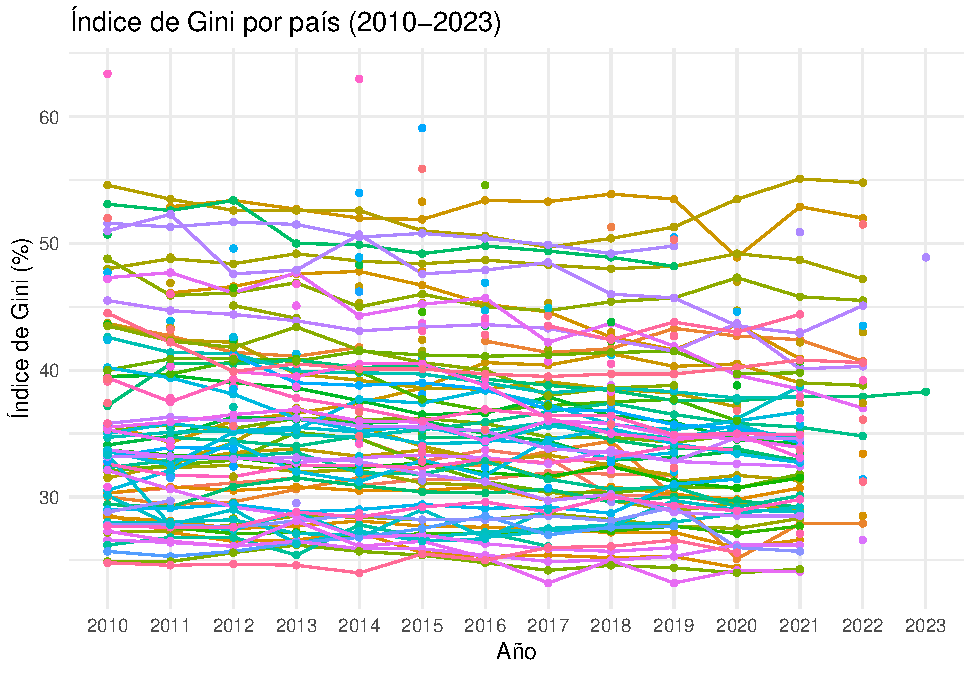
\includegraphics{Informe_files/figure-latex/unnamed-chunk-3-1.pdf}

Se observa una notable estabilidad en los valores del índice de Gini
desde el año 2010 hasta el 2019, con algunos cambios más importantes
identificados en el año 2020. También realizando un análisis
longitudinal exploratorio, la variabilidad entre países es la dominante,
con muy poca variabilidad intra. Esto se puede ver en el gráfico de
perfiles individuales con las lineas de cada país prácticamente
constantes. Cabe destacar que se tienen pocos datos en los años
posteriores a la pandemia. Por lo tanto, se decide utilizar el dato de
Gini de 2019 o el más reciente disponible de cada país, hasta el año
2010 como máximo, para garantizar que todos los datos sean lo más
actualizados posibles, anulando el efecto de la pandemia y la poca
cantidad de observaciones de los años más recientes 2022 y 2023.

Finalmente, en la nueva dimensión denominada Libertad, los datos
utilizados son los del informe creado por Freedom House. La base de
datos con todos los puntajes de los indicadores desde 2013 se encuentra
en la página web de la organización.

\subsection{Links de descarga de
bases:}\label{links-de-descarga-de-bases}

\begin{enumerate}
\def\labelenumi{\arabic{enumi}.}
\item
  Programa de las Naciones Unidas para el Desarrollo. (2022).
  Documentation and Downloads. Human Development Reports.
  \url{https://hdr.undp.org/data-center/documentation-and-downloads}
  (consultado en junio de 2024).
\item
  World Health Organization. (2020). Healthy Life Expectancy (HALE)
  Data. WHO. \url{https://apps.who.int/gho/data/node.main.HALE?lang=en}
  (consultado en junio de 2024).
\item
  Banco Mundial. (2024). GINI Index. World Bank Data.
  \url{https://datos.bancomundial.org/indicator/SI.POV.GINI} (consultado
  en junio de 2024).
\item
  Freedom House. (2024). Freedom in the World.
  \url{https://freedomhouse.org/report/freedom-world} (consultado en
  junio de 2024).
\end{enumerate}

\subsection{Bibliografía}\label{bibliografuxeda}

\begin{enumerate}
\def\labelenumi{\arabic{enumi}.}
\item
  Banco Mundial. (2024). GINI Index. World Bank Data.
  \url{https://datos.bancomundial.org/indicator/SI.POV.GINI}
\item
  Eustat. (2023). Índice de Desarrollo Humano por Indicadores según
  Países 2022.
  \url{https://es.eustat.eus/elementos/ele0013500/ti_indice-de-desarrollo-humano-por-indicadores-segun-paises-2022/tbl0013566_c.html}
\item
  Freedom House. (2024). Freedom in the World 2024.
  \url{https://freedomhouse.org/report/freedom-world}
\item
  Instituto Nacional de Estadística (España). (2023). Esperanza de Vida
  en Buena Salud. INE.
  \url{https://www.ine.es/ss/Satellite?L=es_ES&c=INESeccion_C&cid=1259926378861&p=\%5C&pagename=ProductosYServicios\%2FPYSLayout&param1=PYSDetalle&param3=1259924822888}
\item
  Programa de las Naciones Unidas para el Desarrollo. (2010). Human
  Development Report 2010.
  \url{https://hdr.undp.org/content/human-development-report-2010}
\item
  Programa de las Naciones Unidas para el Desarrollo. (2019). Human
  Development Report 2019.
  \url{https://hdr.undp.org/content/human-development-report-2019}
\item
  Programa de las Naciones Unidas para el Desarrollo. (2023). Notas
  Técnicas sobre el Cálculo de los Índices de Desarrollo Humano.
  \url{https://www.undp.org/sites/g/files/zskgke326/files/2023-09/notas_tecnicas.pdf}
\item
  Programa de las Naciones Unidas para el Desarrollo. (2024). About
  Human Development. Human Development Reports.
  \url{https://hdr.undp.org/about/human-development}
\item
  Sullivan, D. (2014). Guide to Using the Sullivan Method for
  Calculating Healthy Life Expectancy.
  \url{https://reves.site.ined.fr/fichier/s_rubrique/20182/sullivan.guide.pre.final.oct2014.en.pdf}
\item
  Verywell Health. (2022). Understanding Healthy Life Expectancy.
  \url{https://www.verywellhealth.com/understanding-healthy-life-expectancy-2223919\#toc-how-hale-is-calculated}
\item
  World Health Organization. (2020). Healthy Life Expectancy (HALE)
  Metadata.
  \url{https://cdn.who.int/media/docs/default-source/gho-documents/metadata/hale-metadata.pdf?sfvrsn=4f47fd43_1&download=true}
\item
  World Health Organization. (2020). Life Expectancy and Healthy Life
  Expectancy. WHO.
  \url{https://www.who.int/data/gho/data/themes/topics/indicator-groups/indicator-group-details/GHO/life-expectancy-and-healthy-life-expectancy}
\end{enumerate}

\end{document}
